\documentclass[conference]{IEEEtran}
\IEEEoverridecommandlockouts
% The preceding line is only needed to identify funding in the first footnote. If that is unneeded, please comment it out.
\usepackage{cite}
\usepackage{natbib}
\usepackage{float}
\usepackage{amsmath,amssymb,amsfonts}
\usepackage{algorithmic}
\usepackage{graphicx}
\usepackage{textcomp}
\usepackage{hyperref}
\usepackage{xcolor}


\usepackage{booktabs, makecell}

\hypersetup{
    colorlinks=true,
    linkcolor=blue,
    filecolor=magenta,      
    urlcolor=blue,
    pdftitle={Overleaf Example},
    pdfpagemode=FullScreen,
    }


\def\BibTeX{{\rm B\kern-.05em{\sc i\kern-.025em b}\kern-.08em
    T\kern-.1667em\lower.7ex\hbox{E}\kern-.125emX}}
\begin{document}

\title{CENG318 Human Computer Interaction\\Group 14 Final Project Report\\Spring 2023\\
    {Project Title: Herbify}\\
%{\footnotesize \textsuperscript{*}Note: Sub-titles are not captured in Xplore and
%should not be used}
}
\makeatletter
\newcommand{\linebreakand}{%
  \end{@IEEEauthorhalign}
  \hfill\mbox{}\par
  \mbox{}\hfill\begin{@IEEEauthorhalign}
}
\makeatother

\author{\IEEEauthorblockN{Yasir Duman}
\IEEEauthorblockA{\textit{Computer Engineering} \\
\textit{280201101}}
\and
\IEEEauthorblockN{Halil İbrahim Buğday}
\IEEEauthorblockA{\textit{Computer Engineering} \\
\textit{280201094 }}
\and
\IEEEauthorblockN{Kerem Yavuz Şenyurt}
\IEEEauthorblockA{\textit{Computer Engineering} \\
\textit{290201100}}
\linebreakand
\IEEEauthorblockN{Berkan Gönülsever}
\IEEEauthorblockA{\textit{Computer Engineering} \\
\textit{270201064}}
\and
\IEEEauthorblockN{Gökay Gülsoy}
\IEEEauthorblockA{\textit{Computer Engineering} \\
\textit{270201072}}
}

\maketitle

\begin{abstract}
Many people encounter  different type of plants in daily life or a flower photo in digital environment. For us people, it is a bit headache to distinguish a plant from others. Even if we know the plant’s name, we probably don’t know much about its features. In this project named Herbify, Users will be able to obtain fast accurate and reliable information about plants without the need to search for a long time on the Internet. In Herbify, users need to upload a photo of the plant they wish to gain knowledge about and then they can access lots of useful information, such as plant care, their origins and general knowledge. Herbify uses artificial intelligence and huge set of data related with plants to identify a plant in the photo with high accuracy. Apart from comprehensive information related with plants Herbify also provide different resources for adequate reading. Agile methodology is used to develop Herbify where every user can discover new information while they are having fun.
\end{abstract}

\begin{IEEEkeywords}
plant identification, artificial intelligence, gamification
\end{IEEEkeywords}

\section{Introduction}
Plants existed before humanity and play crucial role in life. plants serve as the foundation of food chains and produces oxygen which is essential for the survival of all beings, including humans.Throughout history, humans have relied on plants in numerous ways. We look back to the past, humans used plants as food, medical, dressing and tool. Today, plants are still play an important role in our life, however everybody does not share the same level of interest in plants. For ordinary people, it can sometimes be difficult to recognize a plant with a similar appearance to others. To help people who want to indetify a plant and who want to know more about plants, we developed web application named Herbify

Herbify is a web application that utilizes object recognition to help users identify different types of plants. With Herbify, users can easily snap a photo of any plant they come across and get instant results about its name, features, and potential uses.

However, traditional plant identification apps often lack user engagement and fail to provide additional features that users may find useful. Herbify seeks to solve this problem by incorporating gamification elements into the app, such as a points system for correct plant identifications and a social feature for users to share their findings with others.

Additionally, Herbify aims to provide users with comprehensive information about each plant, including its medicinal properties, growing conditions, and ecological significance. By combining cutting-edge technology with engaging design, Herbify strives to make plant identification both educational and entertaining for users of all ages and backgrounds.

\section{Literature Review}
Plant identification has become easier with the development of numerous plant identification websites and mobile applications.
In this section, several plant identification apps/websites including PlantNet \cite{PlantNet}, PlantSnap \cite{PlantSnapMobileApp} \cite{PlantSnapWebsite}, Blossom \cite{GooglePlayBlossom}, plant.id \cite{PlantId}, iNaturalist Seek \cite{iNaturalist}, LeafSnap \cite{LeafSnap}, Google Lens \cite{GoogleLens}, Bing \cite{Bing}, and Flora Incognita \cite{FloraIncognita} will be reviewed in context of their plant identification sucess rates , user reviews and pricings.
 The apps studied are listed in Table 1. One of the apps was discarded early on because some of its features were not testable.

\subsection{Plant Identification Success}
Plant identification success is crucial for the efficiency and effectiveness of plant identification tools.
Several studies have compared the identification success rates of different plant identification tools.
One study conducted by \cite{AOBP} compared the identification accuracy  different plant identification apps including PlantNet , PlantSnap , iNaturalist Seek and LeafSnap.
The study found that Plant.id had the highest identification success average score of 69.8 followed by Google Lens with 63.4, while Bing had the lowest success average score of 16.3. Average scores obtained for the first identification by each of the apps for each sub grouping of the samples whether by plant type or by plant part with the number of samples in each subset. Results can be seen in Table 2.
However, the success rate of these tools may vary depending on various factors such as the quality of the image, the complexity of the plant, and the accuracy of the database.

Another research study (Author, Year) investigated the relationship between identification success of species (percentage of images identified to the species level) and the number of training images used for the Flora Incognita machine learning algorithm. The number of training images was presented on a logarithmic scale on the graph, and a log-transformation was applied prior to Pearson correlation analysis. The findings of this study revealed a positive correlation between the number of training images and the identification success rate. As the number of training images increased, the algorithm's ability to accurately identify plant species improved. 

These research findings contribute to the understanding of the factors influencing plant identification success and highlight the significance of robust training data in machine learning algorithms. By incorporating a large and diverse image database, our app aims to improve the plant identification success rate and provide users with more accurate and reliable results.

\begin{figure}[H]
\centerline{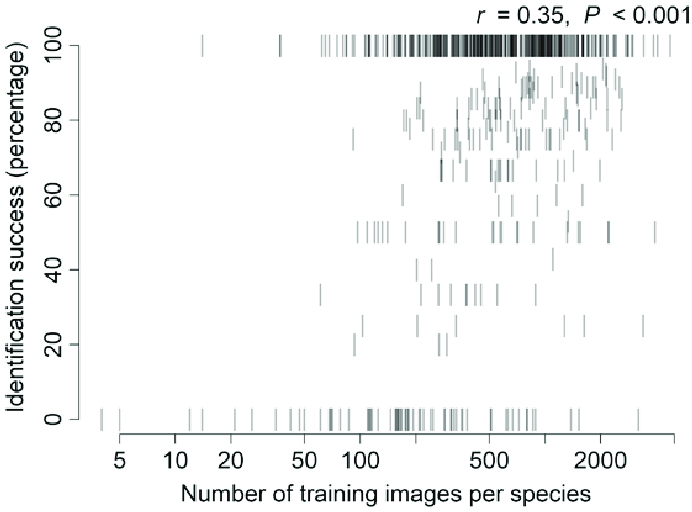
\includegraphics[width=0.48 \textwidth]{images/eeeee.png}}
\end{figure}



\subsection{User Reviews}
User reviews provide valuable insights into the user experience of plant identification tools.
The user reviews of different plant identification tools were analyzed to determine their overall user satisfaction.
Users of plant identification apps have reported mixed experiences with the apps. While some users praise the apps for their accuracy and ease of use, others complain about poor performance, wrong identifications, and design issues. For example, some users have reported that PlantSnap fails to identify certain plants, and others have criticized the app's subscription model. Similarly, some users have found the identification suggestions provided by iNaturalist Seek to be inaccurate or unhelpful, while others have praised the app's user-friendly interface. Design issues have also been noted, with some users finding the user interface of certain apps to be confusing or difficult to navigate.
\subsection{Price}
Pricing is an essential factor to consider when choosing a plant identification tool.
While some plant identification apps are free to download and install on a user's device, most of them require in-app purchases or subscriptions to unlock full functionality. This means that while the basic features of the app may be available for free, users may need to pay to access additional features or content. It is important to note that several identification apps require some form of in-app purchase or subscription in order to continue using the app beyond the initial free download.
\newline 
\subsection{Conclusion}
According to research and examinations about the apps and websites, it is seen that  common problems with the plant identification apps are, poor user experience, relatively high  prices and plant identification success. Herbify aims to solves these problems with better design, computer vision approaches and additional features integrated with gamification.


\begin{figure}[H]
\centerline{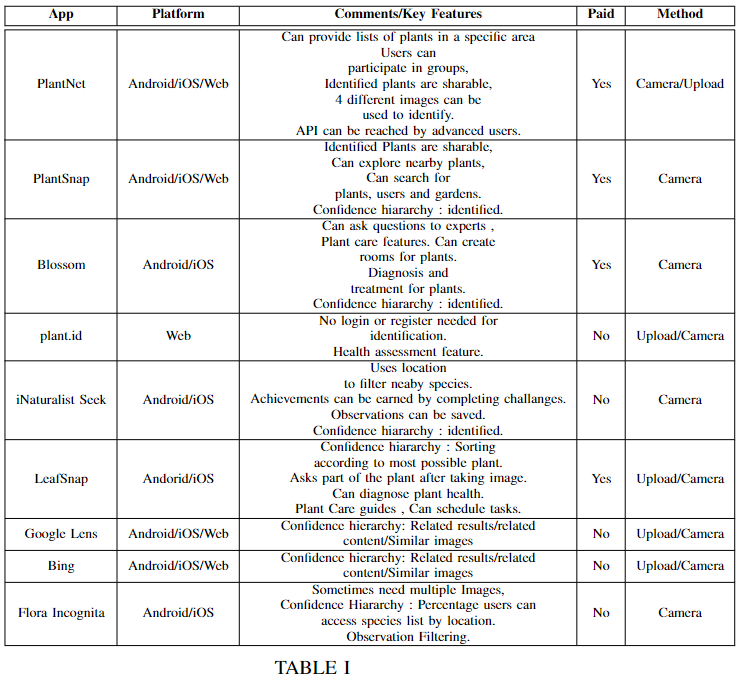
\includegraphics[width=0.48 \textwidth]{images/table1.png}}
\end{figure}

\begin{figure}[H]
\centerline{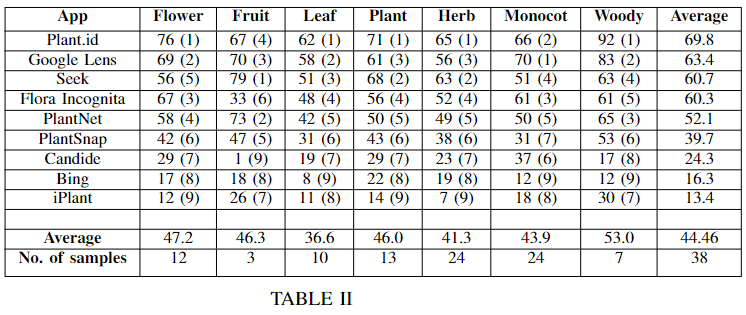
\includegraphics[width=0.48 \textwidth]{images/table2.png}}
\end{figure}





\section{Methodology}

 \subsection{AI Development}
    \subsubsection{Data Collection}The first step we did is collecting a large dataset of plant images. We did obtain these images from kaggle.com. We did ensure that the dataset includes a diverse range of plant species, including those that are commonly found in different regions.
    \subsubsection{Data Preprocessing}Before using the dataset for training the deep learning model, we did preprocess the images to ensure that they were of high quality and consistent. If there were irrelevant or noisy images we removed them then we standardized the size (224*224) and orientation of the images to fit the model we use.
    \subsubsection{Model Training}We used VGG16 convolution neural network architecture \cite{FlowerImageClassification} to create our model. We did split the dataset into training, validation, and testing sets. We used approximately 4000 images for training, 1 image for validation, and 100 images for testing and so the model was trained to recognize the unique features of each plant species and classify them accurately.
    \subsubsection{Model Optimization}After training the model, we did try to optimize its performance. We did evaluate the model's performance on the testing with new images.

\subsection{Backend Development}
The Backend Development phase focused on the server-side implementation and functionality of our application. This involved designing the database, developing the necessary APIs, and ensuring smooth communication between the frontend and backend components. The backend development process consisted of the following key steps:
    \subsubsection{Design}
    During the Design phase, we carefully planned and defined the architecture and functionality of our application. This phase played an important role in shaping the overall structure and behavior of the system. The Design phase involved the following key components:
        \paragraph{Database Design}
        We designed the database architecture to store and manage relevant data efficiently.
	This involved identifying the  necessary tables, defining their relationships, and establishing data schemas.
    \paragraph{Use Case Development}
    We created detailed Use Cases to outline various scenarios and interactions between users and the application.
	These Use Cases provided a clear understanding of how users would interact with the system and the expected outcomes in different situations.
    \paragraph{UML Sequence Diagrams}
    We prepared UML Sequence Diagrams to visually represent the flow of actions and messages between different components in the application.
	These diagrams helped to visualize the dynamic behavior of the system and understand the sequence of events during specific processes.
 \paragraph{Test Case Development}
 We developed  Test Cases to validate the functionality of the application.
	Test Cases covered various scenarios, ensuring that the application performed as intended and met the specified requirements.

 \subsubsection{Backend Implementation}
We have implemented the necessary backend functionality to enable efficient data exchange, secure authentication, and various operations within our application.
To ensure secure access to the application, we have implemented authentication mechanisms. These mechanisms involve user authentication and authorization processes, safeguarding user data and preventing unauthorized access.
Our backend implementation includes  functionalities for retrieving plant information from the system.
In addition, we have implemented features to securely store user data within the backend system. These mechanisms ensure the safe storage and management of user information and preferences.

\subsubsection{Security Measures}
We implemented necessary security measures to protect user data and ensure the integrity of the system.
This involved authentication mechanisms and data encryption.

        
\subsection{UI Development} 
 Once the model is optimized, we have started to design a user-friendly user interface template by considering the Nielsen’s 10 Heuristics for our tool.We first created paper prototypes for each of our pages that will be on our website. Then we improve these paper prototypes. Then we createdFirst we create HTML files to structure our webpages and
its content then we create css files to style and layout our
webpages. We use flask web framework to give our website
functionalities. We choose flask framework because it provides
useful tools and features that digital prototypes on the Canva website based on the paper prototypes.

\subsection{Integration}
Once the backend implementation was completed, we proceeded to integrate the developed backend functionalities with the frontend components. This integration aimed to establish seamless interaction between the user interface, backend system, and AI model. The integration process involved handling incoming requests, processing data, and sending appropriate responses back to the frontend.

\subsection{User Evaluation}We conducted an evaluation of our system, gathering feedback from users on various aspects including user experience, system functionalities, and plant identification success.
The evaluation aimed to assess the user satisfaction and system integrity.



\section{Experimental Results}
Show and explain preliminary experiments that have done so far with their corresponding setups and results. 

\subsection{Paper Prototype}

1) Version 0


\begin{figure}[H]
\centerline{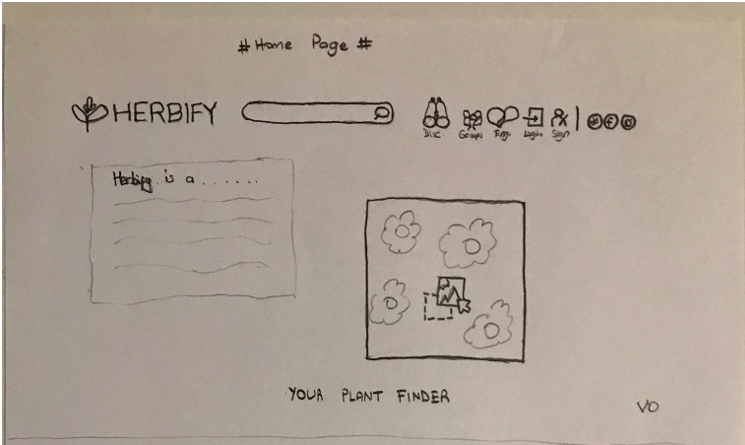
\includegraphics[width=0.48 \textwidth]{images/home0.png}}
\caption{Home Page Paper Prototype Version 0}
\label{fig:graph1}
\end{figure}

\begin{figure}[H]
\centerline{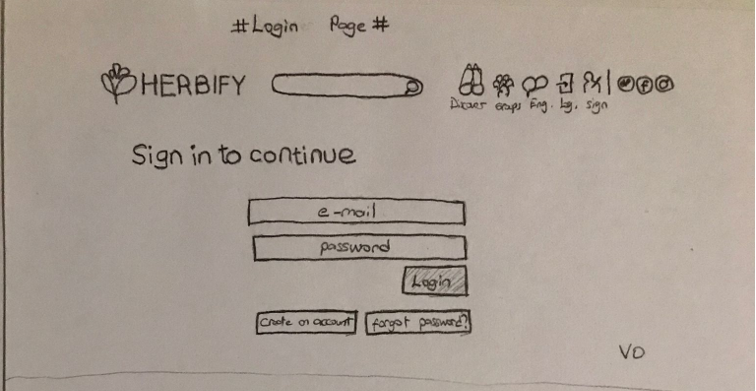
\includegraphics[width=0.48 \textwidth]{images/login0.png}}
\caption{Login Page Paper Prototype Version 0}
\label{fig:graph1}
\end{figure}

\begin{figure}[H]
\centerline{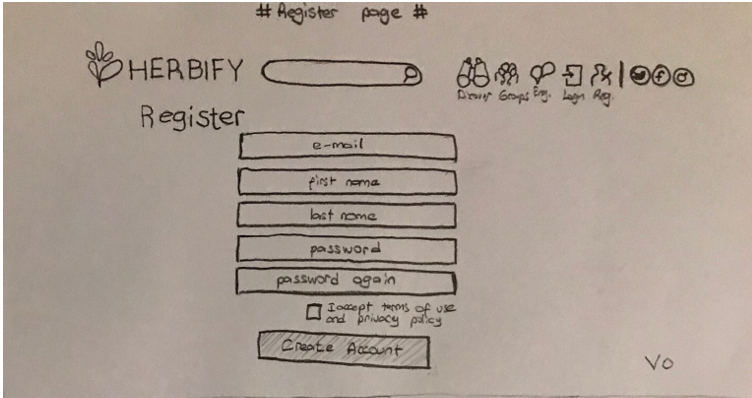
\includegraphics[width=0.48 \textwidth]{images/register0.png}}
\caption{Register Page Paper Prototype Version 0}
\label{fig:graph1}
\end{figure}

\begin{figure}[H]
\centerline{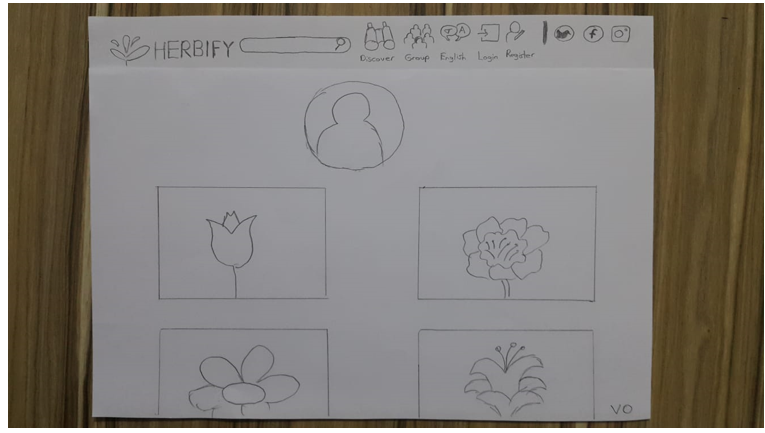
\includegraphics[width=0.48 \textwidth]{images/profile0.png}}
\caption{Profile Page Paper Prototype Version 0}
\label{fig:graph1}
\end{figure}

\begin{figure}[H]
\centerline{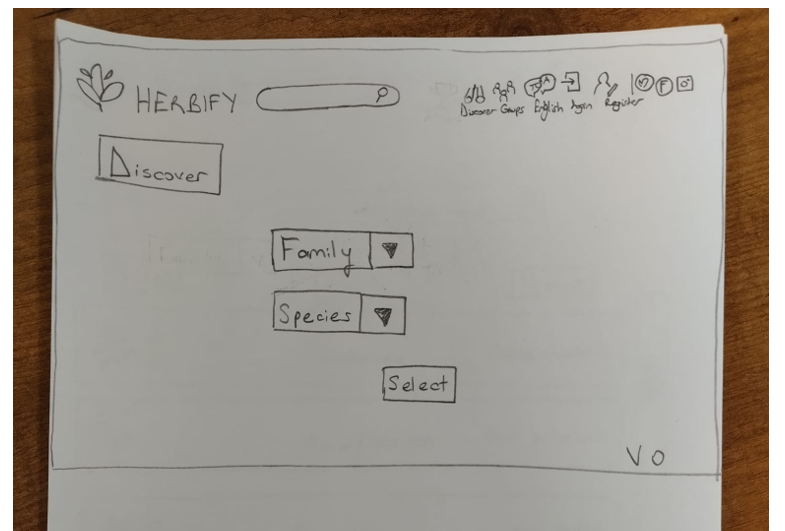
\includegraphics[width=0.48 \textwidth]{images/discover0.png}}
\caption{Discover Page Paper Prototype Version 0}
\label{fig:graph1}
\end{figure}


\begin{figure}[H]
\centerline{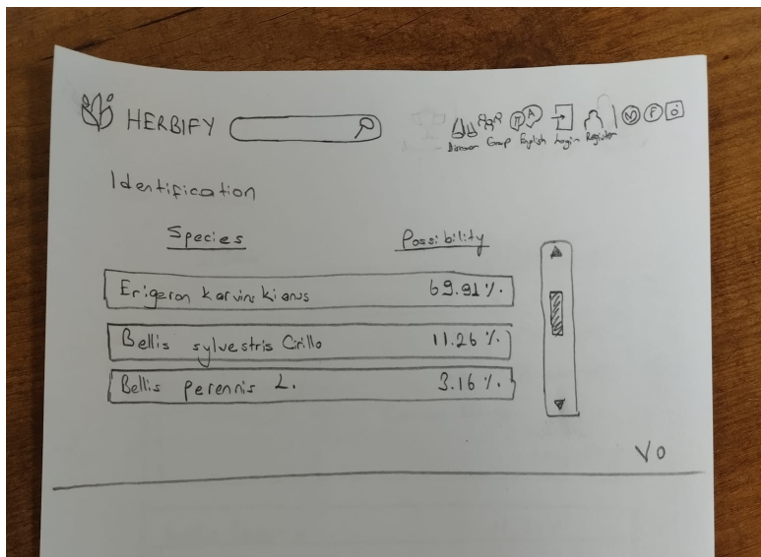
\includegraphics[width=0.48 \textwidth]{images/identification0.png}}
\caption{Identification Paper Prototype Version 0}
\label{fig:graph1}
\end{figure}


\begin{figure}[H]
\centerline{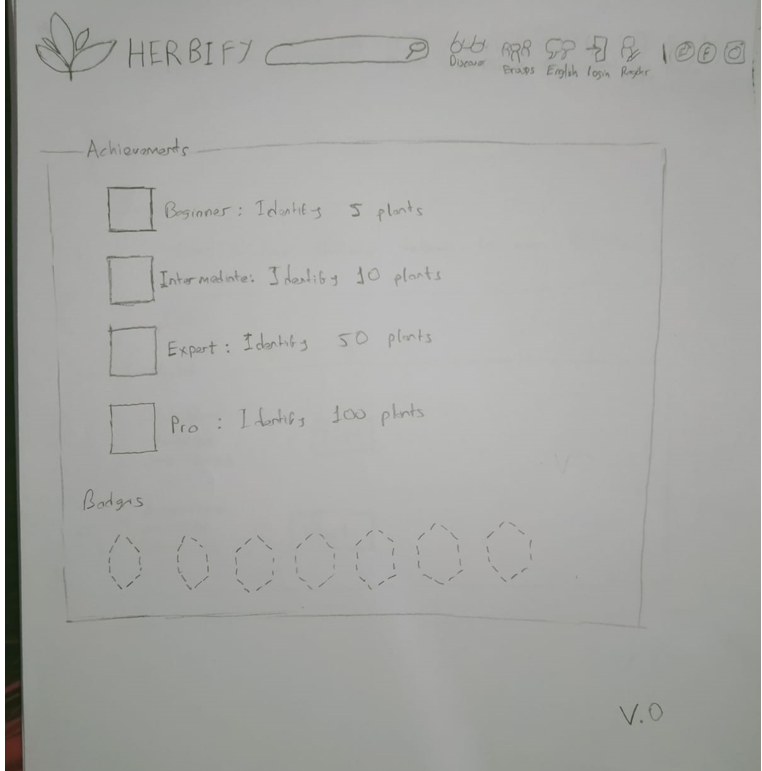
\includegraphics[width=0.48 \textwidth]{images/achivements.png}}
\caption{Achievements Paper Prototype Version 0}
\label{fig:graph1}
\end{figure}


\begin{figure}[H]
\centerline{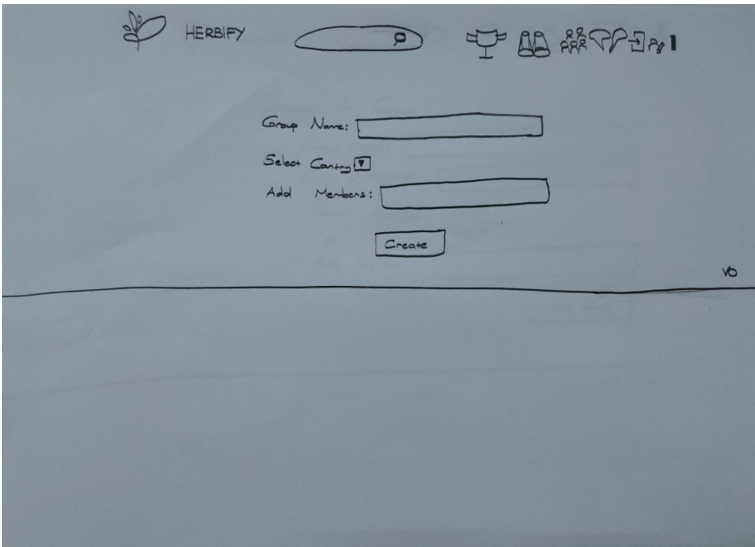
\includegraphics[width=0.48 \textwidth]{images/create0.png}}
\caption{Create Group Paper Prototype Version 0}
\label{fig:graph1}
\end{figure}


\begin{figure}[H]
\centerline{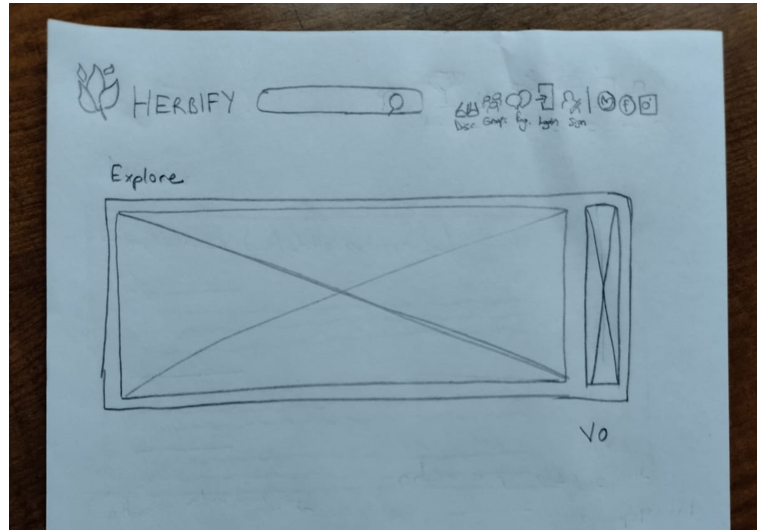
\includegraphics[width=0.48 \textwidth]{images/explore0.png}}
\caption{Explore Paper Prototype Version 0}
\label{fig:graph1}
\end{figure}

\begin{figure}[H]
\centerline{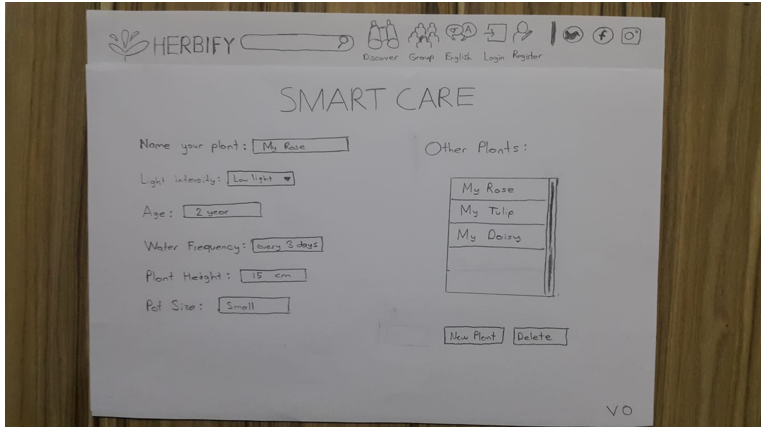
\includegraphics[width=0.48 \textwidth]{images/smartcare0.png}}
\caption{Smart Care Prototype Version 0}
\label{fig:graph1}
\end{figure}


\begin{figure}[H]
\centerline{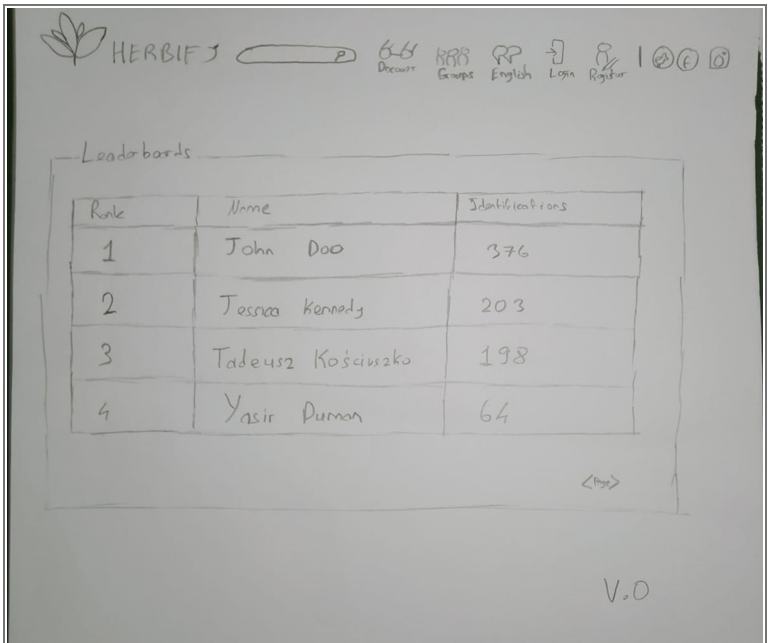
\includegraphics[width=0.48 \textwidth]{images/leader0.png}}
\caption{Leader Prototype Version 0}
\label{fig:graph1}
\end{figure}


\begin{figure}[H]
\centerline{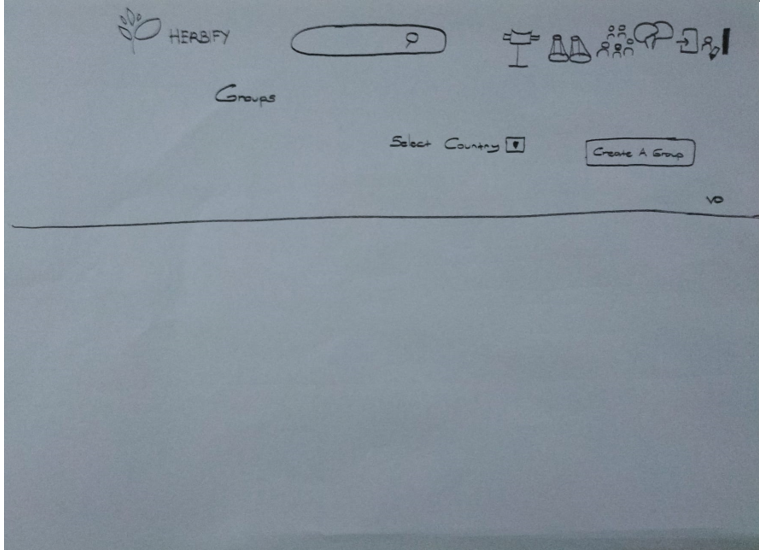
\includegraphics[width=0.48 \textwidth]{images/groups0.png}}
\caption{Groups Prototype Version 0}
\label{fig:graph1}
\end{figure}

\begin{figure}[H]
\centerline{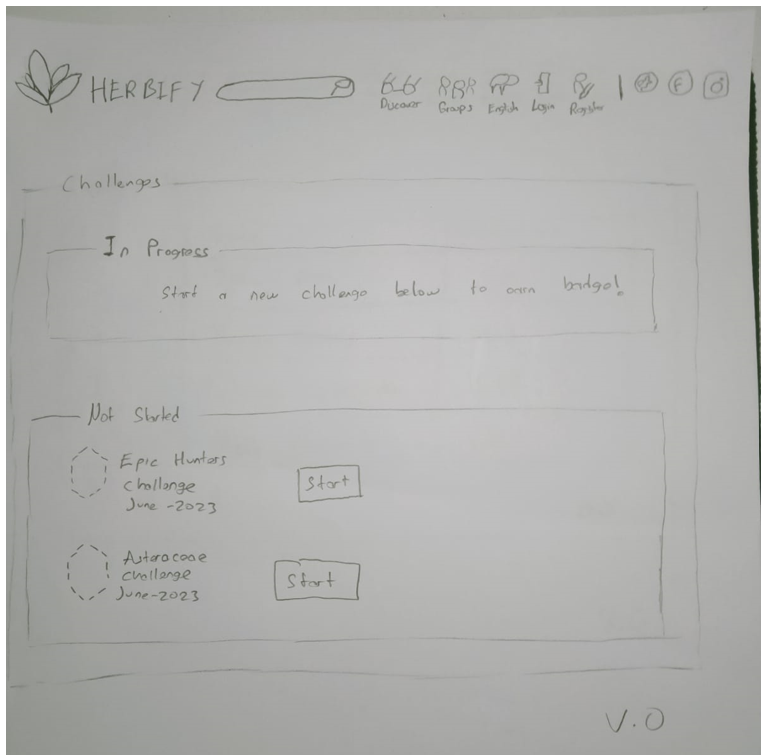
\includegraphics[width=0.48 \textwidth]{images/challenges0.png}}
\caption{Challenges Prototype Version 0}
\label{fig:graph1}
\end{figure}
}



2) Version 1:

\begin{figure}[H]
\centerline{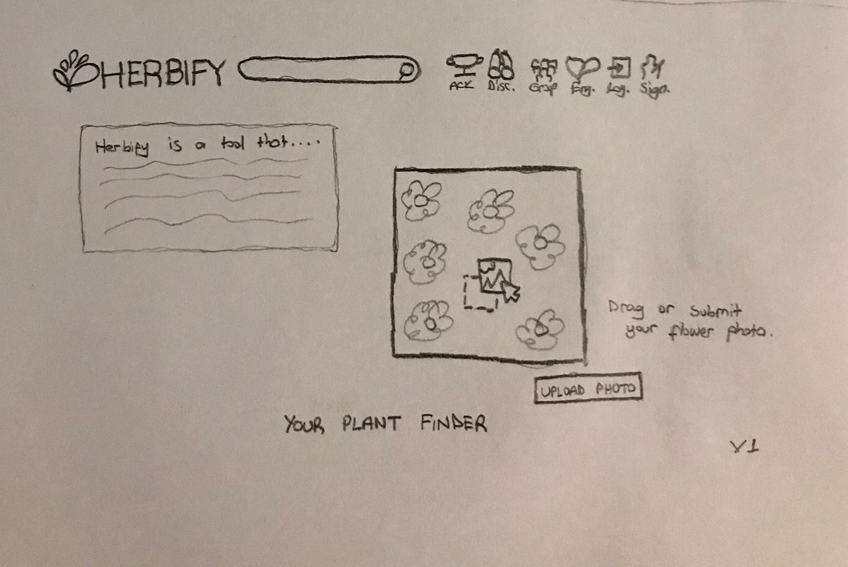
\includegraphics[width=0.48 \textwidth]{images/home-pp1.png}}
\caption{Home Page Paper Prototype Version 1}
\label{fig:graph1}
\end{figure}


\begin{figure}[H]
\centerline{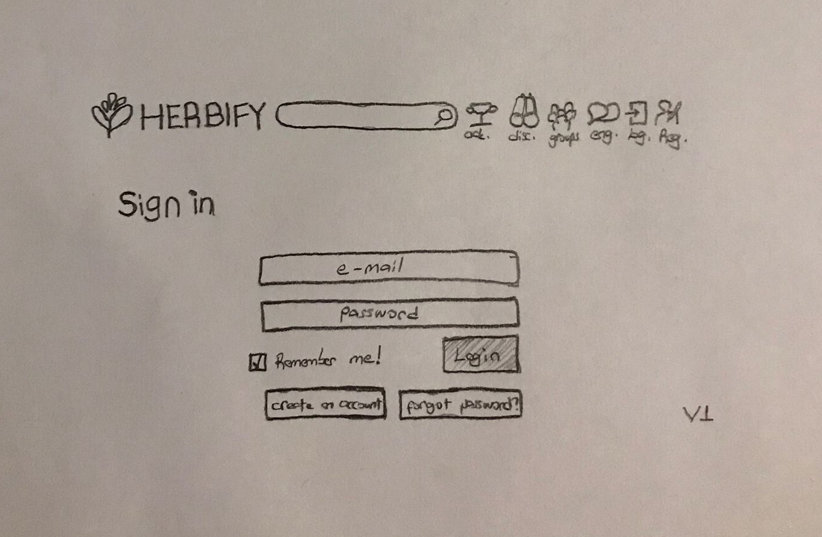
\includegraphics[width=0.48 \textwidth]{images/login-pp1.png}}
\caption{Login Page Paper Prototype Version 1}
\label{fig:graph1}
\end{figure}


\begin{figure}[H]
\centerline{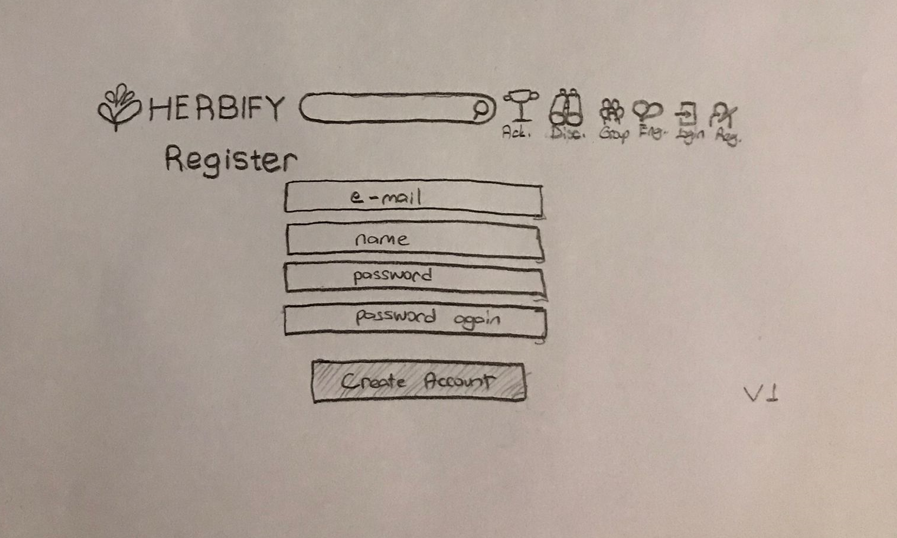
\includegraphics[width=0.48 \textwidth]{images/register-pp1.png}}
\caption{Register Page Paper Prototype Version 1}
\label{fig:graph1}
\end{figure}

\begin{figure}[H]
\centerline{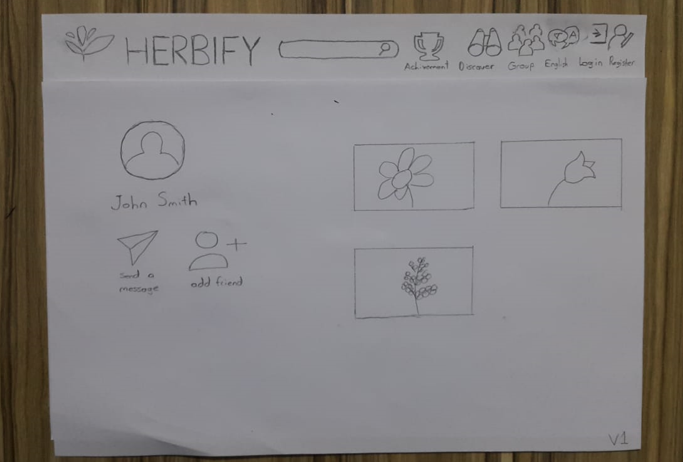
\includegraphics[width=0.48 \textwidth]{images/profile-pp1.png}}
\caption{Profile Page Paper Prototype Version 1}
\label{fig:graph1}
\end{figure}


\begin{figure}[H]
\centerline{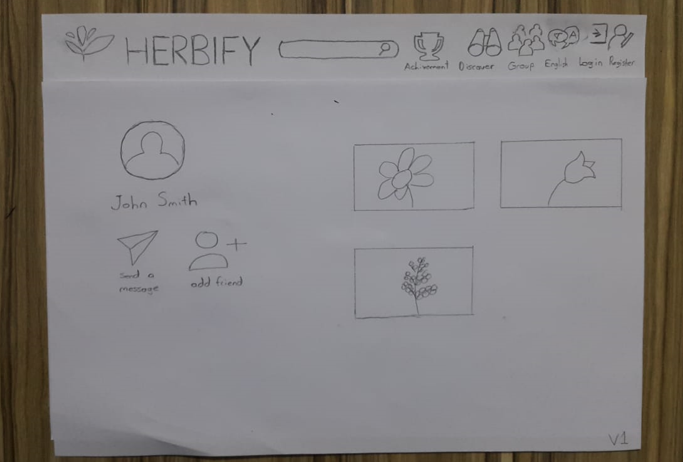
\includegraphics[width=0.48 \textwidth]{images/profile-pp1.png}}
\caption{Profile Page Paper Prototype Version 1}
\label{fig:graph1}
\end{figure}

\begin{figure}[H]
\centerline{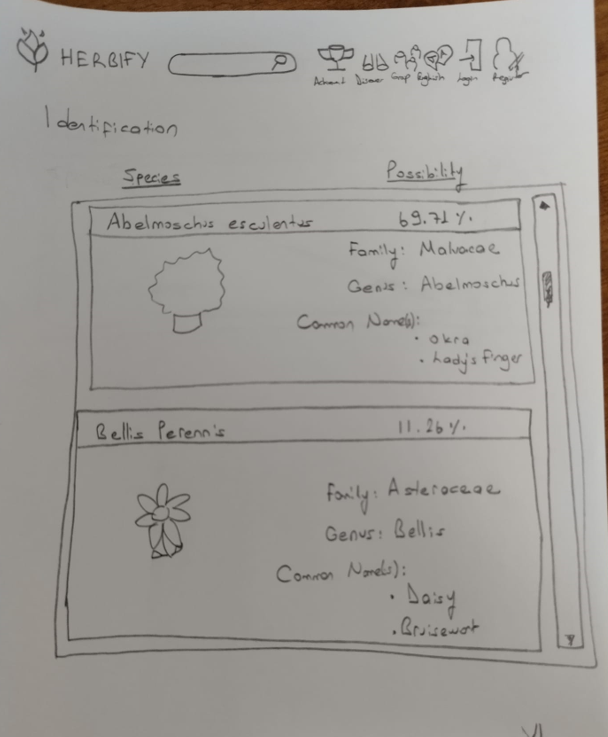
\includegraphics[width=0.48 \textwidth]{images/identification-pp1.png}}
\caption{Identification Page Paper Prototype Version 1} 
\label{fig:graph1}
\end{figure}


\begin{figure}[H]
\centerline{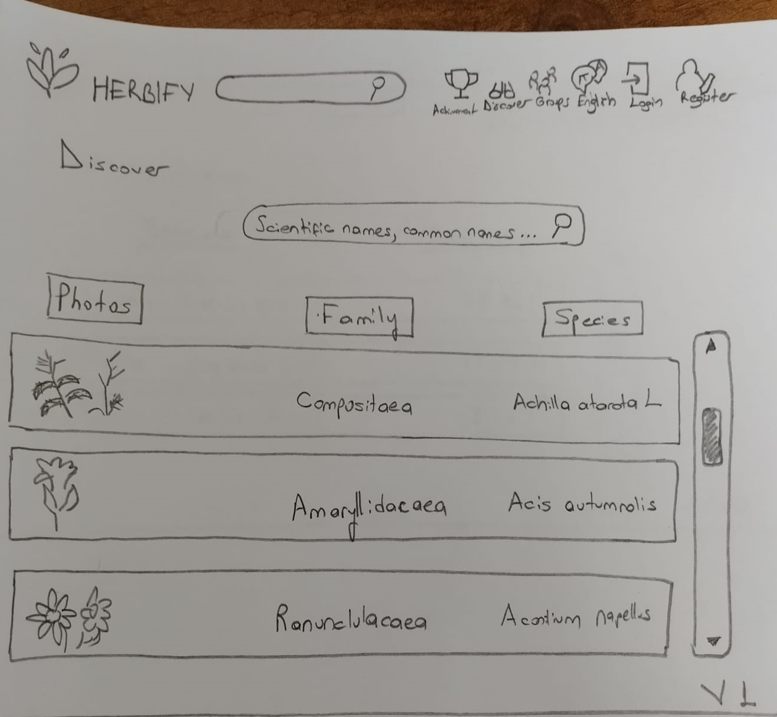
\includegraphics[width=0.48 \textwidth]{images/discover-pp1.png}}
\caption{Discover Paper Prototype Version 1}
\label{fig:graph1}
\end{figure}


\begin{figure}[H]
\centerline{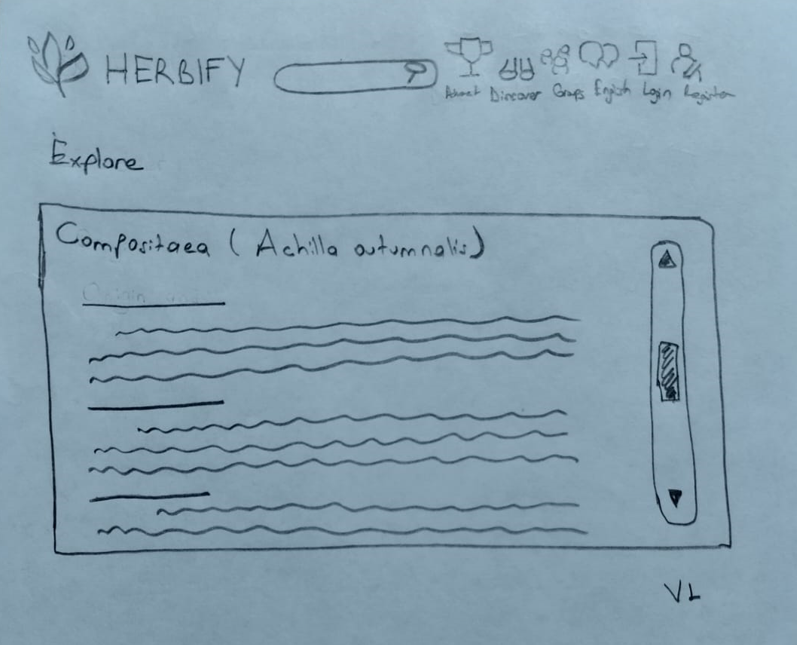
\includegraphics[width=0.48 \textwidth]{images/explore-pp1.png}}
\caption{Explore Paper Prototype Version 1}
\label{fig:graph1}
\end{figure}

\begin{figure}[H]
\centerline{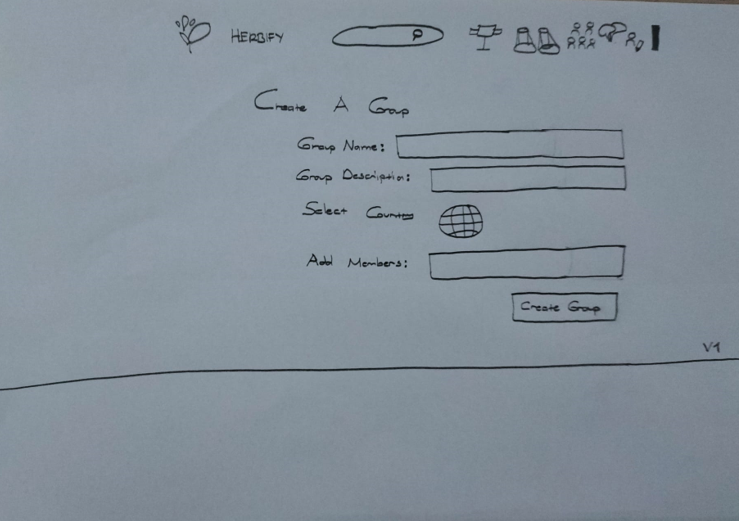
\includegraphics[width=0.48 \textwidth]{images/creategroups-pp1.png}}
\caption{Create Groups Paper Prototype Version 1}
\label{fig:graph1}
\end{figure}


\begin{figure}[H]
\centerline{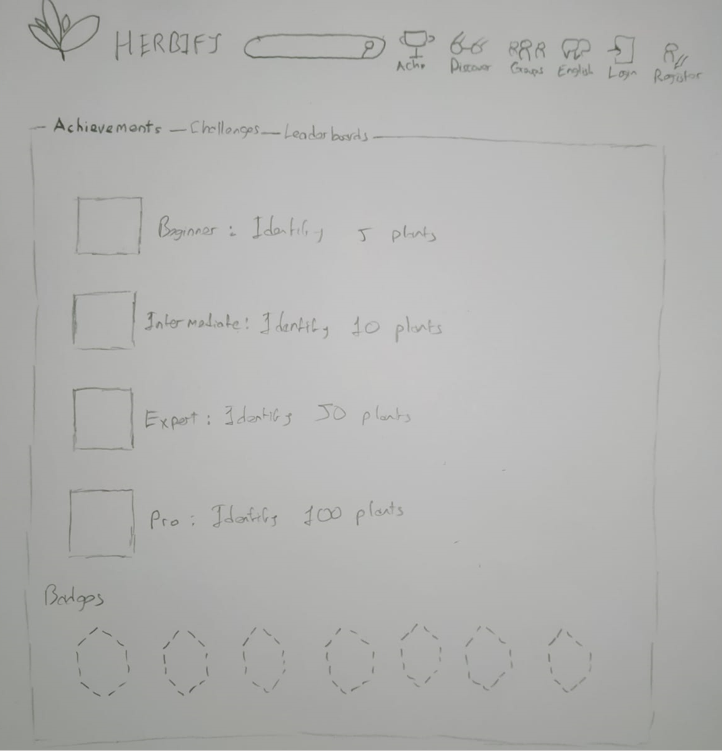
\includegraphics[width=0.48 \textwidth]{images/achivements-pp1.png}}
\caption{Achievements Paper Prototype Version 1}
\label{fig:graph1}
\end{figure}



\begin{figure}[H]
\centerline{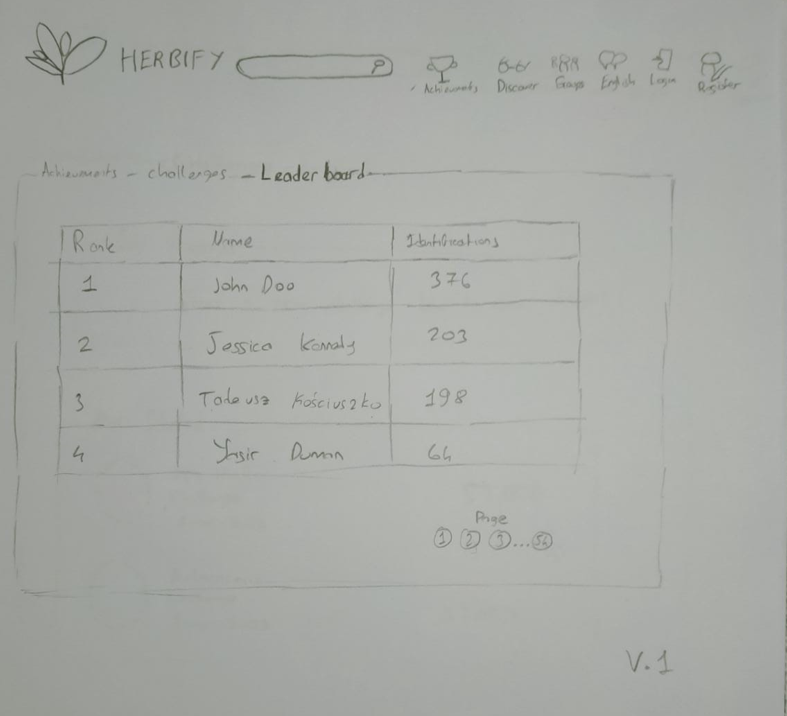
\includegraphics[width=0.48 \textwidth]{images/leaderboard-pp1.png}}
\caption{Leaderboard Paper Prototype Version 1}
\label{fig:graph1}
\end{figure}


\subsection{Digital Design}

1) Version 0

\begin{figure}[H]
\centerline{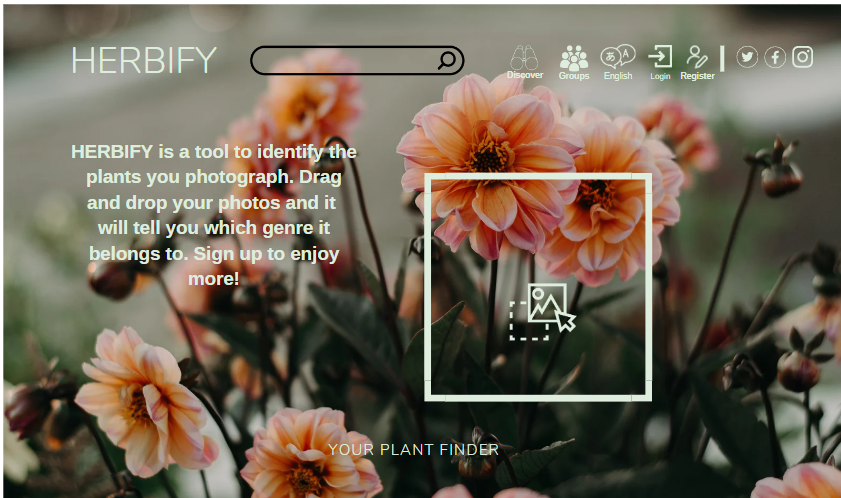
\includegraphics[width=0.48 \textwidth]{images/homev0(identification).png}}
\caption{Home Page Version 0}
\label{fig:graph1}
\end{figure}


\begin{figure}[H]
\centerline{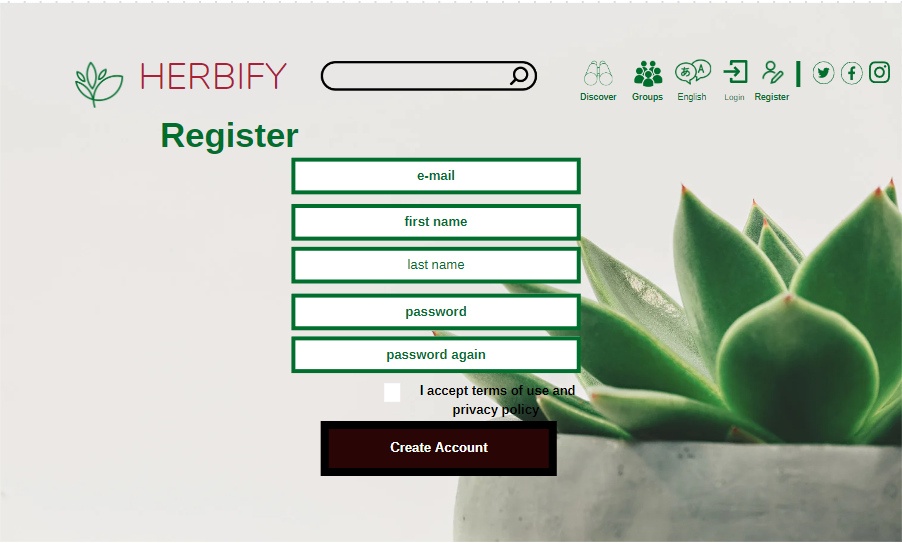
\includegraphics[width=0.48 \textwidth]{images/registerv0.png}}
\caption{Register Page Version 0}
\label{fig:graph1}
\end{figure}

\begin{figure}[H]
\centerline{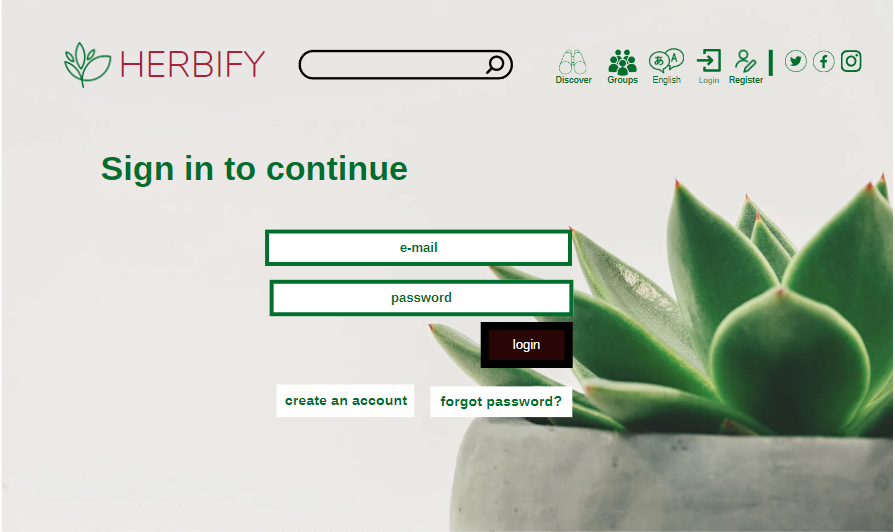
\includegraphics[width=0.48 \textwidth]{images/sign-inv0.png}}
\caption{Sign-in Page Version 0}
\label{fig:graph1}
\end{figure}

\begin{figure}[H]
\centerline{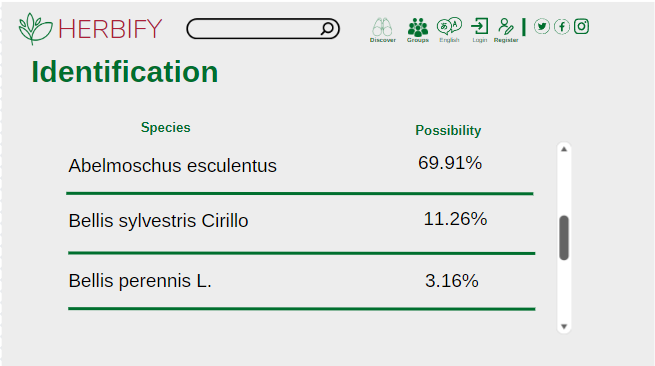
\includegraphics[width=0.48 \textwidth]{images/identificationv0.png}}
\caption{Identification Page Version 0}
\label{fig:graph1}
\end{figure}

\begin{figure}[H]
\centerline{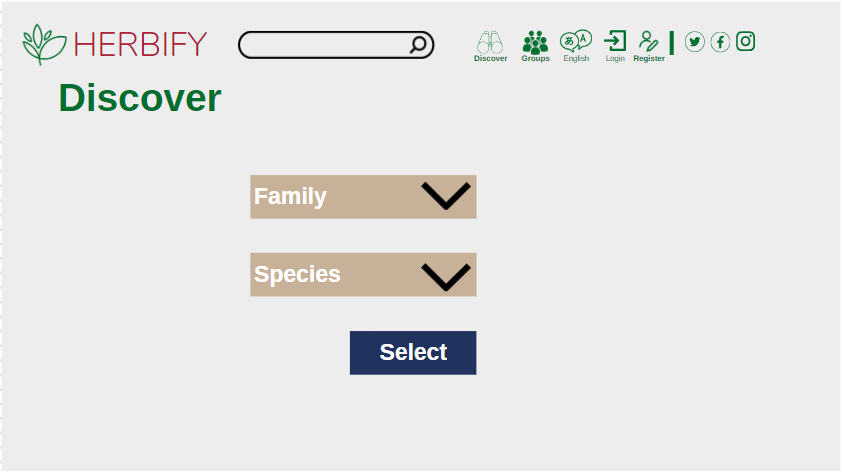
\includegraphics[width=0.48 \textwidth]{images/discoverv0.png}}
\caption{Discover Page Version 0}
\label{fig:graph1}
\end{figure}


\begin{figure}[H]
\centerline{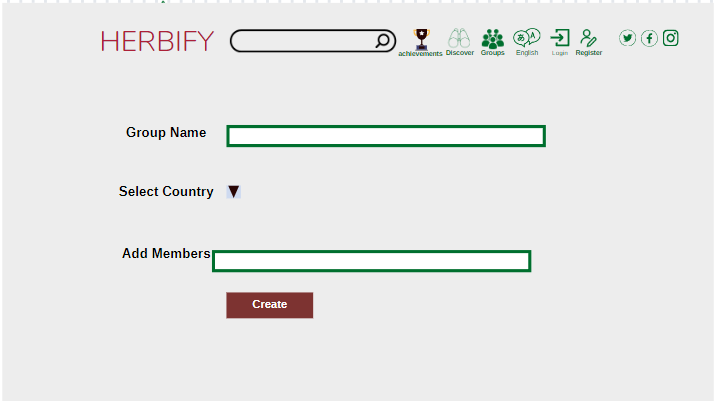
\includegraphics[width=0.48 \textwidth]{images/creategroupv0.png}}
\caption{Create Group Page Version 0}
\label{fig:graph1}
\end{figure}


\begin{figure}[H]
\centerline{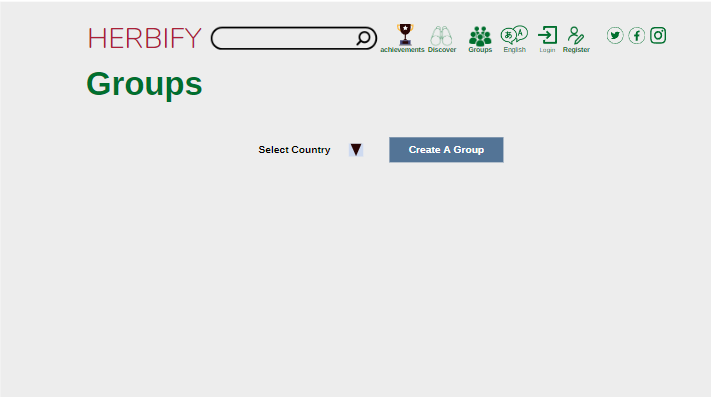
\includegraphics[width=0.48 \textwidth]{images/joingroupv0.png}}
\caption{Join Group Page Version 0}
\label{fig:graph1}
\end{figure}



\begin{figure}[H]
\centerline{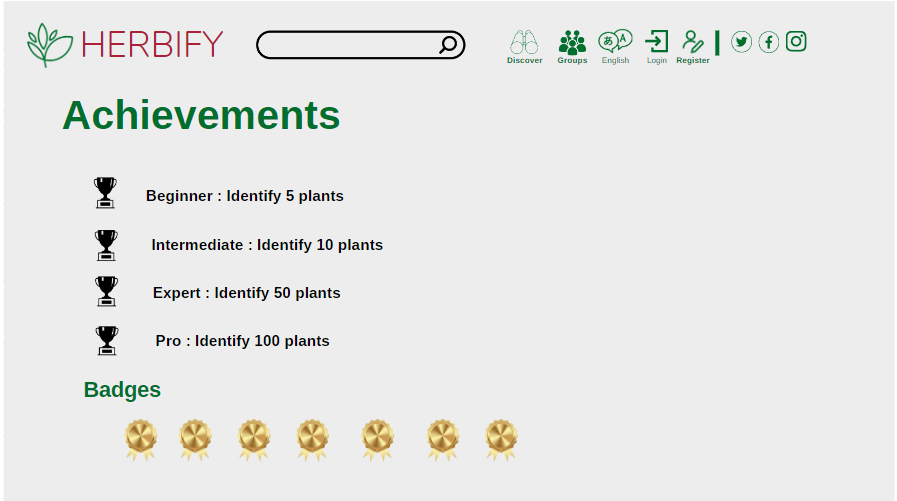
\includegraphics[width=0.48 \textwidth]{images/achivementsV0.png}}
\caption{Achivement Page Version 0}
\label{fig:graph1}
\end{figure}


\begin{figure}[H]
\centerline{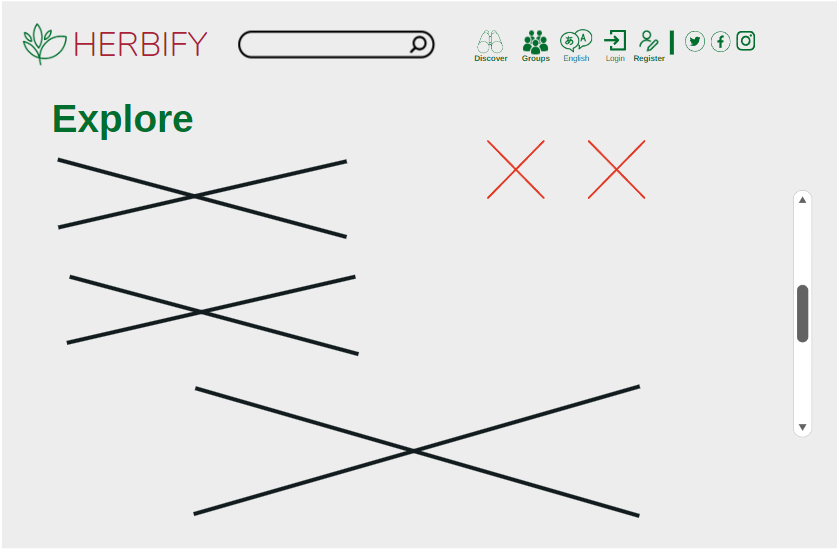
\includegraphics[width=0.48 \textwidth]{images/exploreV0.png}}
\caption{Explore Page Version 0}
\label{fig:graph1}
\end{figure}


\begin{figure}[H]
\centerline{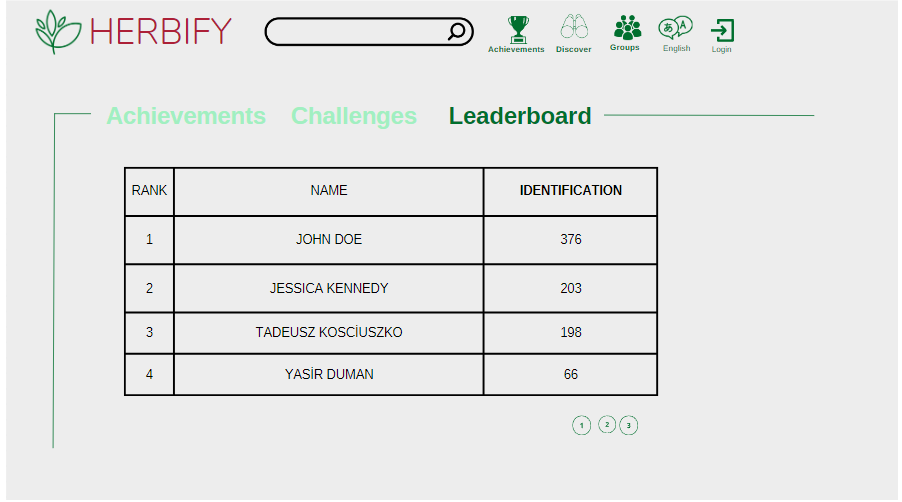
\includegraphics[width=0.48 \textwidth]{images/leaderboardv0.png}}
\caption{Leader Board Page Version 0}
\label{fig:graph1}
\end{figure}


\begin{figure}[H]
\centerline{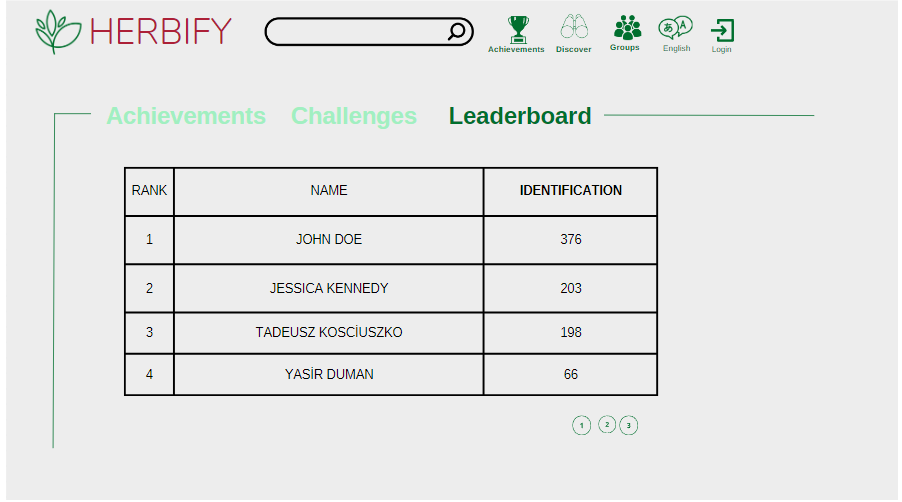
\includegraphics[width=0.48 \textwidth]{images/leaderboardv0.png}}
\caption{Leader Board Page Version 0}
\label{fig:graph1}
\end{figure}

\begin{figure}[H]
\centerline{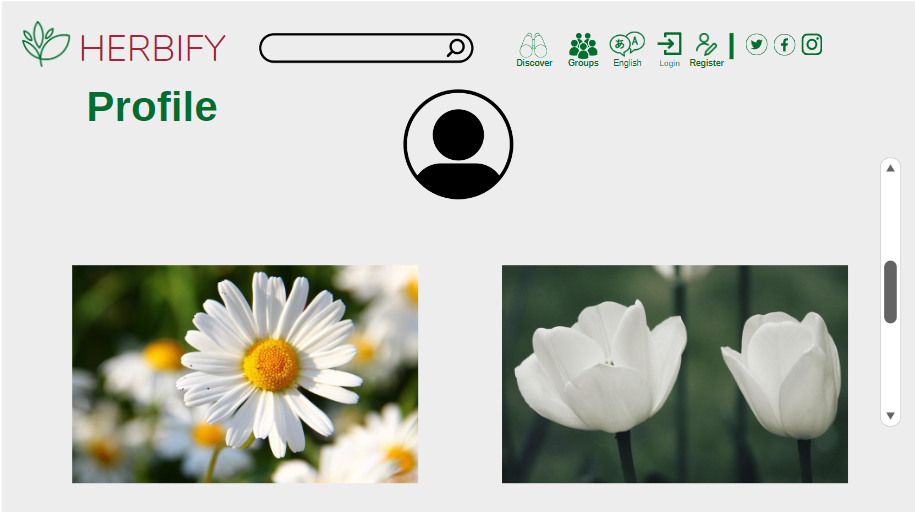
\includegraphics[width=0.48 \textwidth]{images/profilev0.png}}
\caption{Profile Page Version 0}
\label{fig:graph1}
\end{figure}

\begin{figure}[H]
\centerline{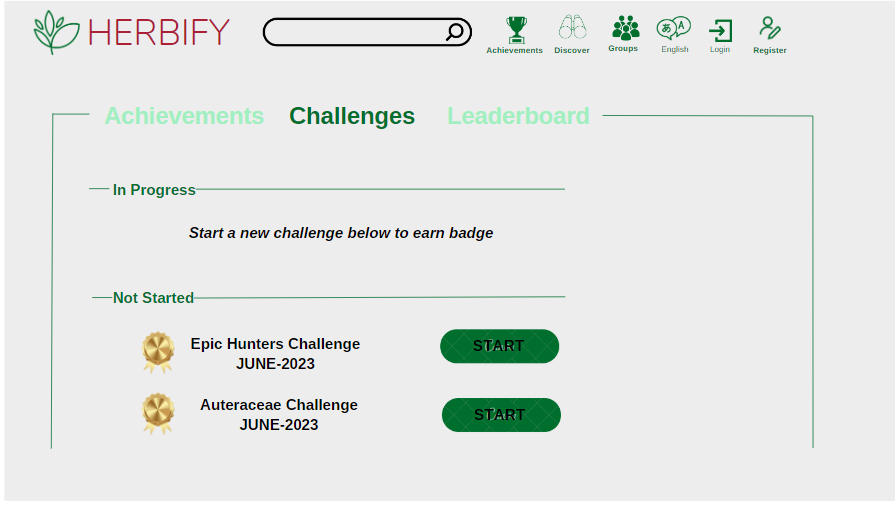
\includegraphics[width=0.48 \textwidth]{images/challengesv0.png}}
\caption{Challenges Page Version 0}
\label{fig:graph1}
\end{figure}


\begin{figure}[H]
\centerline{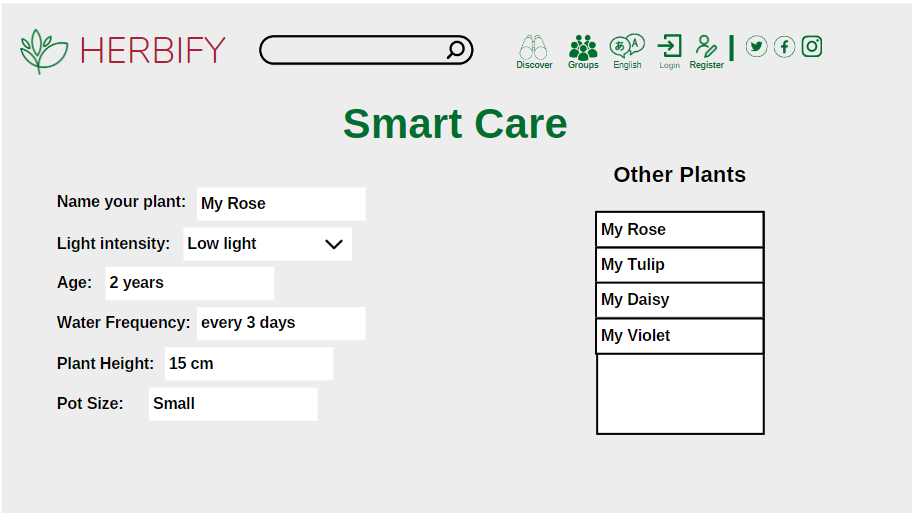
\includegraphics[width=0.48 \textwidth]{images/smartcarev0.png}}
\caption{Smart Care Page Version 0}
\label{fig:graph1}
\end{figure}

2) Version 1


\begin{figure}[H]
\centerline{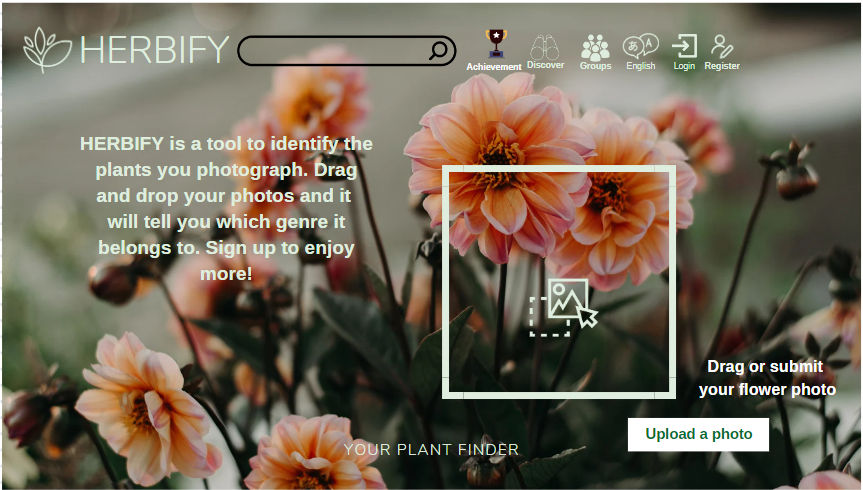
\includegraphics[width=0.48 \textwidth]{images/homev1.png}}
\caption{Home Page Version 1}
\label{fig:graph1}
\end{figure}


\begin{figure}[H]
\centerline{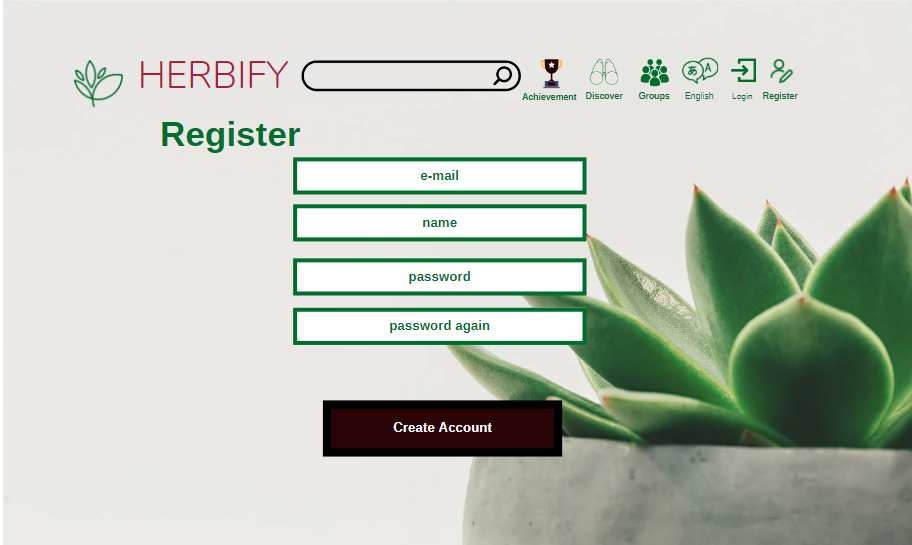
\includegraphics[width=0.48 \textwidth]{images/registerv1.png}}
\caption{Register Page Version 1}
\label{fig:graph1}
\end{figure}


\begin{figure}[H]
\centerline{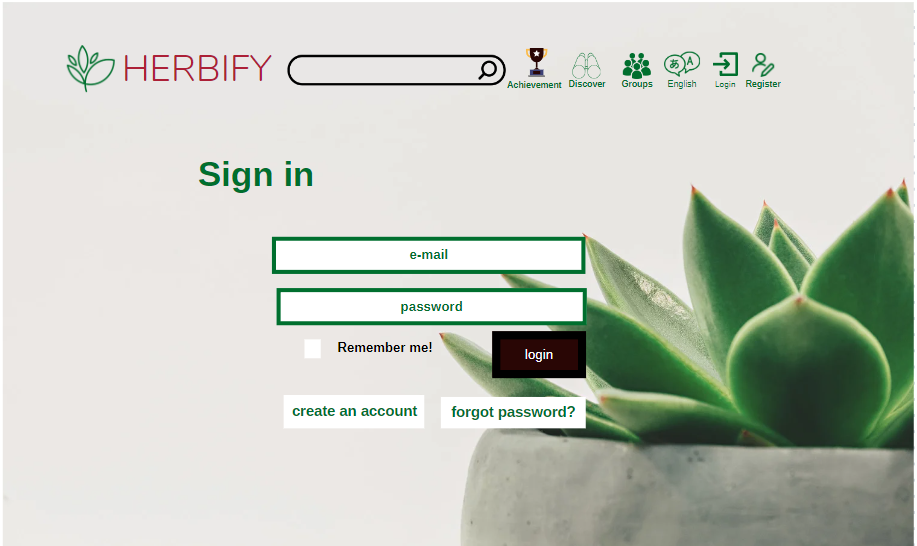
\includegraphics[width=0.48 \textwidth]{images/signinv1.png}}
\caption{Sign-in Page Version 1}
\label{fig:graph1}
\end{figure}


\begin{figure}[H]
\centerline{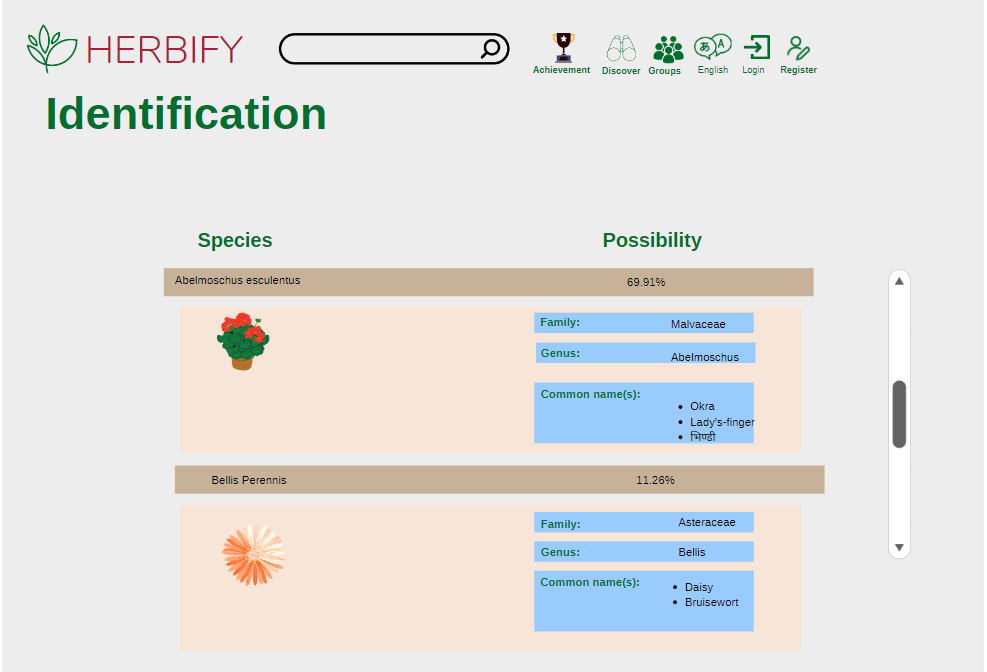
\includegraphics[width=0.48 \textwidth]{images/identificaitonv1.png}}
\caption{Identification Page Version 1}
\label{fig:graph1}
\end{figure}


\begin{figure}[H]
\centerline{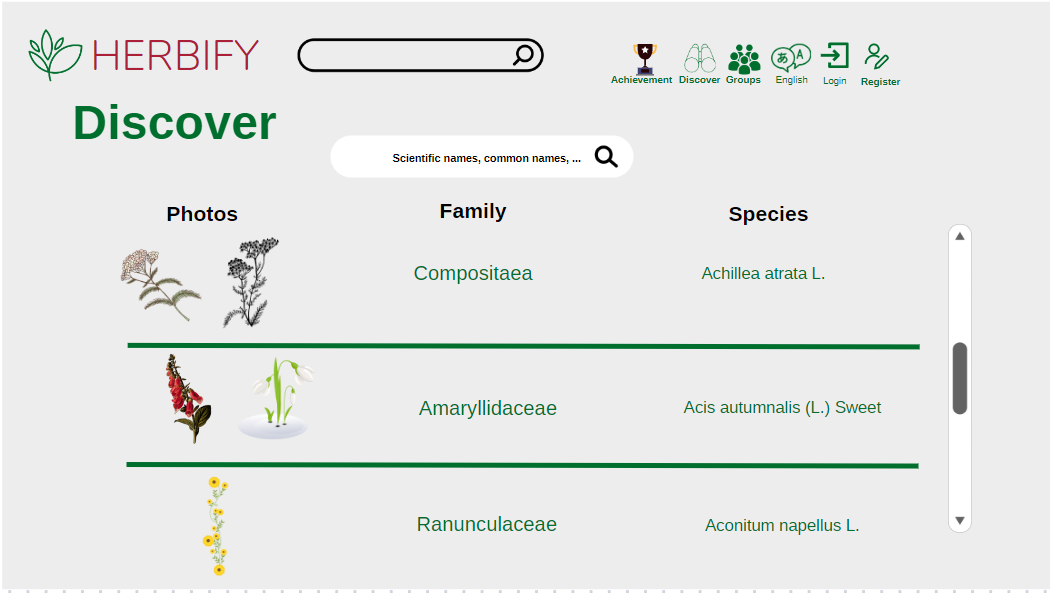
\includegraphics[width=0.48 \textwidth]{images/discoverv1.png}}
    \caption{Discover Page Version 1}
\label{fig:graph1}
\end{figure}



\begin{figure}[H]
\centerline{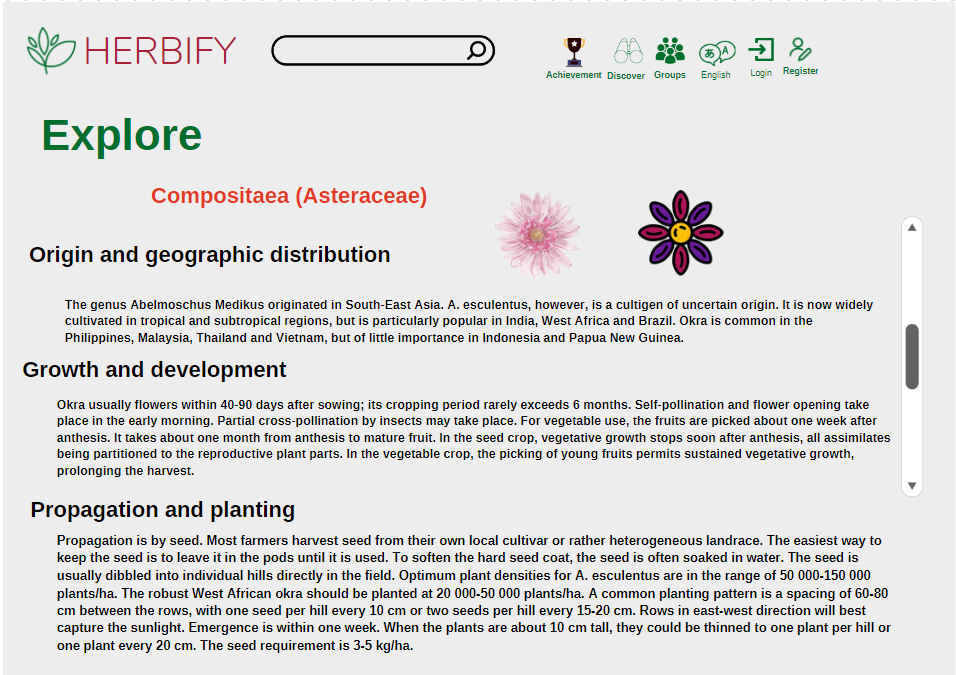
\includegraphics[width=0.48 \textwidth]{images/explorev1.png}}
\caption{Explore Page Version 1}
\label{fig:graph1}
\end{figure}


\begin{figure}[H]
\centerline{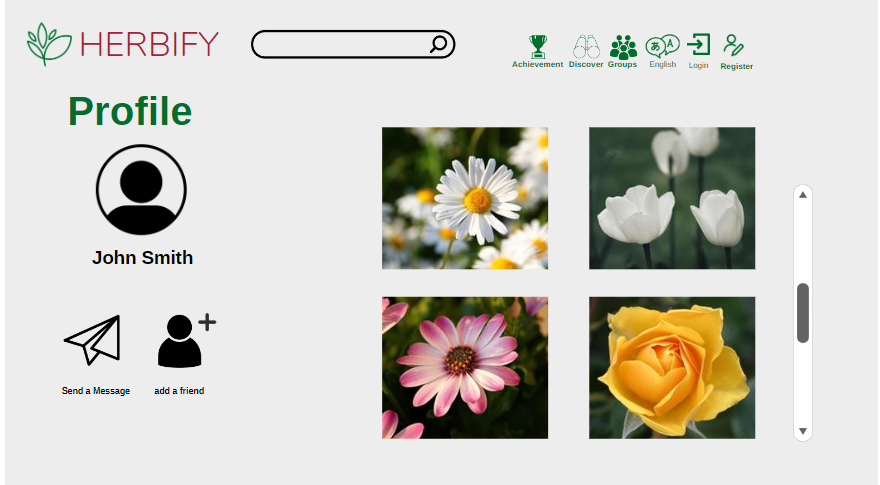
\includegraphics[width=0.48 \textwidth]{images/profilev1.png}}
\caption{Profile Page Version 1}
\label{fig:graph1}
\end{figure}


\begin{figure}[H]
\centerline{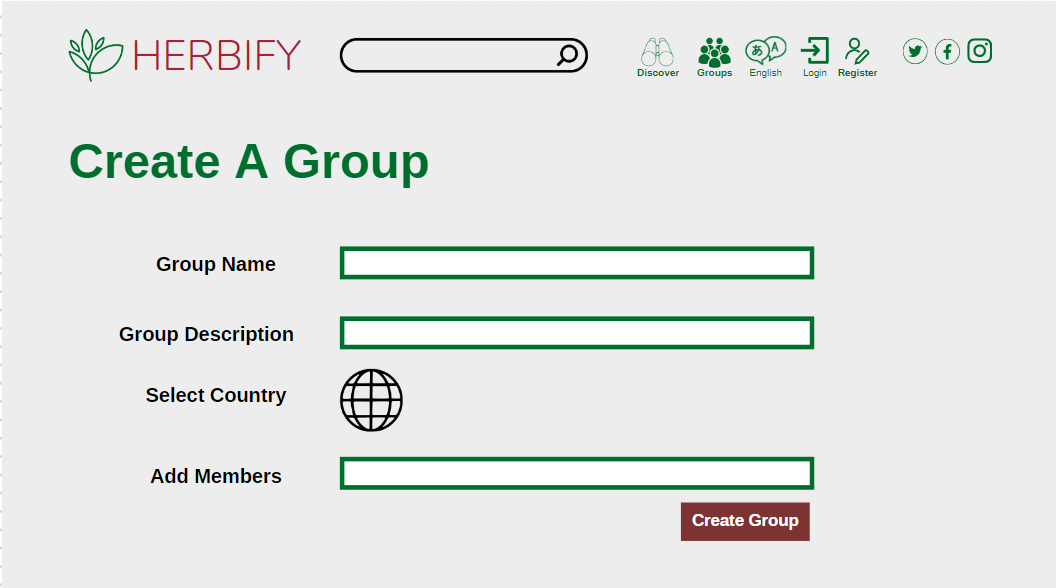
\includegraphics[width=0.48 \textwidth]{images/creategroupv1.png}}
\caption{Create Group Page Version 1}
\label{fig:graph1}
\end{figure}


\begin{figure}[H]
\centerline{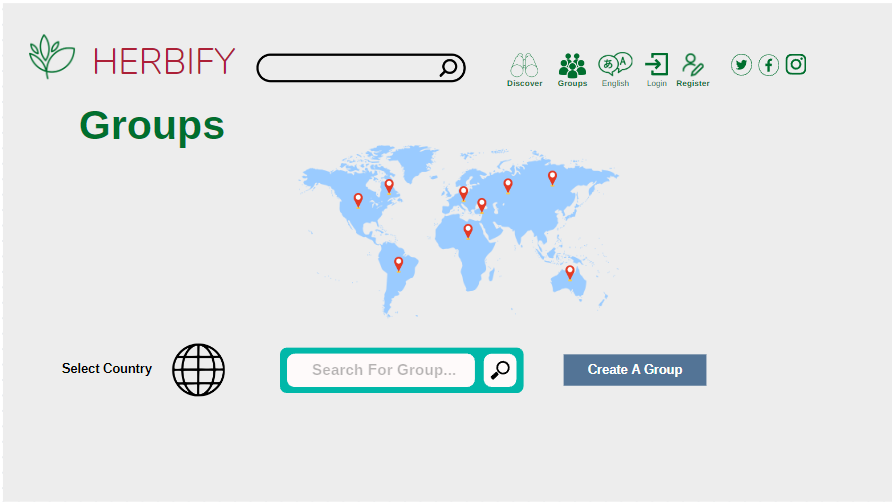
\includegraphics[width=0.48 \textwidth]{images/groupsv1.png}}
\caption{Groups Page Version 1}
\label{fig:graph1}
\end{figure}



\begin{figure}[H]
\centerline{\includegraphics[width=0.48 \textwidth]{images/leaderboardv2.png}}
\caption{Leaderboard Page Version 1}
\label{fig:graph1}
\end{figure}


\begin{figure}[H]
\centerline{\includegraphics[width=0.48 \textwidth]{images/achivementsv1.png}}
\caption{Achievements Page Version 1}
\label{fig:graph1}
\end{figure}


\begin{figure}[H]
\centerline{\includegraphics[width=0.48 \textwidth]{images/challengesv1.png}}
\caption{Challenges Page Version 1}
\label{fig:graph1}
\end{figure}


%\begin{figure}[H]
%\centerline{\includegraphics[width=0.48 \textwidth]{images/smartcarev1.png}}
%\caption{Smart Care Page Version 1}
%\label{fig:graph1}
%\end{figure}



% \begin{figure}[H]
% \centerline{\includegraphics[width=0.48 \textwidth]{images/main_page.png}}
% \caption{Main Page. Users can drag and drop a photo on this page}
% \label{fig:graph6}
% \end{figure}

% \begin{figure}[H]
% \centerline{\includegraphics[width=0.48 \textwidth]{images/sign_in.png}}
% \caption{Sign in Page. Users sign in to the website from this page.}
% \label{fig:graph7}
% \end{figure}

% \begin{figure}[H]
% \centerline{\includegraphics[width=0.48 \textwidth]{images/register.png}}
% \caption{Register Page. Users register on the website from this page.}
% \label{fig:graph8}
% \end{figure}

% \begin{figure}[H]
% \centerline{\includegraphics[width=0.48 \textwidth]{images/discover.png}}
% \caption{Discover Page. Users can search the plants they want to search by using the search bar on this page by their common names, scientific names, genus and species etc.}
% \label{fig:graph9}
% \end{figure}

% \begin{figure}[H]
% \centerline{\includegraphics[width=0.48 \textwidth]{images/explore.png}}
% \caption{Explore Page. Users will be able to access a lot of information such as the family, genus, common names, and growing regions of the plant they are looking for, from this page.}
% \label{fig:graph10}
% \end{figure}

% \begin{figure}[H]
% \centerline{\includegraphics[width=0.48 \textwidth]{images/additional_info.png}}
% \caption{Additional Information Page. On this page, users will find additional reliable information that has been obtained before about the plant}
% \label{fig:graph11}
% \end{figure}

% \begin{figure}[H]
% \centerline{\includegraphics[width=0.48 \textwidth]{images/see all contributor.png}}
% \caption{All Contributors Page. On this page, users will be able to see users who have uploaded photos to our system related to the plant type they are looking for. }
% \label{fig:graph12}
% \end{figure}

% \begin{figure}[H]
% \centerline{\includegraphics[width=0.48 \textwidth]{images/john_smith.png}}
% \caption{Profil Page. On this page, users can review the photos uploaded to our system by users who contributed to our system. They can also send a message to the user or add them as a friend.}
% \label{fig:graph13}
% \end{figure}

% \begin{figure}[H]
% \centerline{\includegraphics[width=0.48 \textwidth]{images/smart care.png}}
% \caption{Smart Care Page. On this page, users can have a smart plant care assistant by entering their growing conditions into the system. The system will send an informative message to users about what to do daily to grow the plant.}
% \label{fig:graph14}
% \end{figure}

% \begin{figure}[H]
% \centerline{\includegraphics[width=0.48 \textwidth]{images/setting care.png}}
% \caption{The system sets the appropriate growing conditions.}
% \label{fig:graph15}
% \end{figure}

% \begin{figure}[H]
% \centerline{\includegraphics[width=0.48 \textwidth]{images/groups.png}}
% \caption{Group Page. Users can see and join previously opened groups here. They can further customize their search by selecting a country.}
% \label{fig:graph16}
% \end{figure}

% \begin{figure}[H]
% \centerline{\includegraphics[width=0.48 \textwidth]{images/create a group.png}}
% \caption{Create A Group. Users can create a group here}
% \label{fig:graph17}
% \end{figure}

\subsection{Future UI Design}

\begin{figure}[H]
\centerline{\includegraphics[width=0.48 \textwidth]{images/Home.jpg}}
\caption{Future Home Page Design}
\label{fig:graph1}
\end{figure}


\begin{figure}[H]
\centerline{\includegraphics[width=0.48 \textwidth]{images/IdentificationFuture.jpg}}
\caption{Future Identification Page Design}
\label{fig:graph1}
\end{figure}


\begin{figure}[H]
\centerline{\includegraphics[width=0.48 \textwidth]{images/AchivementsFuture.jpg}}
\caption{Future Achievements Page Design}
\label{fig:graph1}
\end{figure}


\begin{figure}[H]
\centerline{\includegraphics[width=0.48 \textwidth]{images/GroupsFuture.jpg}}
\caption{Future Groups Page Design}
\label{fig:graph1}
\end{figure}

\begin{figure}[H]
\centerline{\includegraphics[width=0.48 \textwidth]{images/ProfileFuture.jpg}}
\caption{Future Profile Page Design}
\label{fig:graph1}
\end{figure}




\subsection{Photo Recognition AI}

\begin{figure}[H]
\centerline{\includegraphics[width=0.48 \textwidth]{images/ai2.jpg}}
\caption{AI training demonstrated. In this section observed accuracy rates, loss rates, testing rate, training time, batch size and epochs trials. (approximately 4000 photos)}
\label{fig:graph1}
\end{figure}

\begin{figure}[H]
\centerline{\includegraphics[width=0.48 \textwidth]{images/ai1.jpg}}
\caption{After the training is complete, a validation test is performed on a randomly downloaded sunflower image from the internet.}
\label{fig:graph2}
\end{figure}

\begin{figure}[H]
\centerline{\includegraphics[width=0.48 \textwidth]{images/ai3.jpg}}
\caption{After the training is complete, a validation test is performed on a randomly downloaded daisy image from the internet.}
\label{fig:graph3}
\end{figure}

\begin{figure}[H]
\centerline{\includegraphics[width=0.48 \textwidth]{images/ai4.jpg}}
\caption{After the training is complete, a validation test is performed on a randomly downloaded dandelion image from the internet.}
\label{fig:graph4}
\end{figure}

\begin{figure}[H]
\centerline{\includegraphics[width=0.48 \textwidth]{images/ai5.jpg}}
\caption{After the training is complete, a validation test is performed on a randomly downloaded rose image from the internet.}
\label{fig:graph5}
\end{figure}


\subsection{Use Cases}

\begin{figure}[H]
\centerline{\includegraphics[width=0.48 \textwidth]{images/UserLoginUseCse.png}}
\caption{User Login Use Case.}
\label{fig:graph5}
\end{figure}


\begin{figure}[H]
\centerline{\includegraphics[width=0.48 \textwidth]{images/userRegisterUseCase.png}}
\caption{User Register Use Case.}
\label{fig:graph5}
\end{figure}


\begin{figure}[H]
\centerline{\includegraphics[width=0.48 \textwidth]{images/IdentifyUseCase.png}}
\caption{Identification Use Case.}
\label{fig:graph5}
\end{figure}


\subsection{Database Model}

\begin{figure}[H]
\centerline{\includegraphics[width=0.48 \textwidth]{images/classDiagram.png}}
\caption{Database Model Diagram}
\label{fig:graph5}
\end{figure}


\subsection{UML Sequence Diagram}

\begin{figure}[H]
\centerline{\includegraphics[width=0.48 \textwidth]{images/umlRegister.png}}
\caption{Register Sequence Diagram.}
\label{fig:graph5}
\end{figure}


\begin{figure}[H]
\centerline{\includegraphics[width=0.48 \textwidth]{images/umlLogin.png}}
\caption{Login Sequence Diagram.}
\label{fig:graph5}
\end{figure}


\begin{figure}[H]
\centerline{\includegraphics[width=0.48 \textwidth]{images/umlIdentify.png}}
\caption{Identify Sequence Diagram.}
\label{fig:graph5}
\end{figure}


\subsection{Test Cases}

\begin{figure}[H]
\centerline{\includegraphics[width=0.48 \textwidth]{images/loginPositiveTestCase11.png}}
\caption{Login Positive Test Case.}
\label{fig:graph5}
\end{figure}

\begin{figure}[H]
\centerline{\includegraphics[width=0.48 \textwidth]{images/loginNegative11.png}}
\caption{Login Negative Test Case.}
\label{fig:graph5}
\end{figure}



\begin{figure}[H]
\centerline{\includegraphics[width=0.48 \textwidth]{images/userRegisterPositiveTestCase11.png}}
\caption{User Register Positive Test Case.}
\label{fig:graph5}
\end{figure}

\begin{figure}[H]
\centerline{\includegraphics[width=0.48 \textwidth]{images/userRegisterNegativeTestCase11.png}}
\caption{User Register Negative Test Case.}
\label{fig:graph5}
\end{figure}


\begin{figure}[H]
\centerline{\includegraphics[width=0.48 \textwidth]{images/identifyPlantTestCase11.png}}
\caption{Plant Identification Test Case.}
\label{fig:graph5}
\end{figure}


\section{Conclusions and Future Works}
\subsection{Conclusion}
 Herbify is an application that uses photo recognition technology and combines gamification elements to increase user engagement. We mentioned some plant identification apps similar to Herbify and examined them based on their identification success, user reviews, and price. We explained what processes we completed in the frontend, backend and AI side while developing Herbify.  We've included some photos such as paper protoypes, digital design, database model to show the work we've done developing Herbify. \newline

\subsection{Importance}
 Nature, which is a part of our world is in crisis. As a result of global warming, pollution and destruction, the vegetation in our world is decreasing. We think that the way to slow down and stop this is to raise awareness of people and instill a love of nature in them. Our application aims to provide users with information about plants while also ensuring they have an enjoyable time. In this way, we ensure that our application is not disposable, but we make it a part of people's lives where people spend time and taking care of plants. \newline

\subsection{Future Works}
 For the future works, we will make interface designs that users can be more comfortable with and to improve existing interfaces. Another issue we will work on is to improve the photo recognition mechanism, recognize more plants and increase the accuracy rate. In addition to recognizing plants, we are also planning to introduce the feature of recognizing plant diseases with photography.

\section{Weekly Schedule/Project Plan}

Our project schedule is explained in a Gantt Chart. The chart is in the given link with its subtasks: 


\url{https://sharing.clickup.com/9009131277/g/h/4-90090274219-7/3aff0ce79ebf948}


Our aim as five members group is to not overwork ourselves and spread our tasks evenly over the given time span. Our group’s weekly meetings are held online at unspecific times.

\begin{itemize}



  \item \textcolor{green} { Design Analysis (09.03.2023-15.03.2023):\newline\newline
  Task Name: Problem Definition\newline
  Definition: The aim is to find a problem and focus on its solutions. We identified our problem and thought how we can solve the problem. Finally, we decided on our project.\newline
  Current status: Completed.\newline
  Responsible Person: All Team members\newline
  }

  
  \item  \textcolor{green} { Design Analysis (15.03.2023-22.03.2023):\newline\newline
  Task Name: Literature review\newline
  Definition: Review of articles and resources on the subject, the study review process related to the problem.\newline
  Current status: Completed.\newline
  Responsible Person: Gökay Gülsoy, Yasir Duman, Berkan Gönülseven, Kerem Yavuz Şenyurt.\newline\newline
  Task Name: Stages\newline
  Definition: Milestones to be passed for the Project.\newline
  Current status: Completed.\newline
  Responsible Person: Gökay Gülsoy, Berkan Gönülseven\newline\newline
  Task Name: Determines tools\newline
  Definition: Determination of software and hardware tools to be used in the project.\newline
  Current status: Completed.\newline
  Responsible Person: Gökay Gülsoy\newline\newline
  Task Name: Experiments result\newline
  Definition: Designing user interfaces of web pages.\newline
  Current status: Completed.\newline
  Responsible Person: Yasir Duman\newline}
  
  \item \textcolor{green} { AI development (24.03.2023-28.03.2023):\newline\newline
  Task Name: Tools research\newline
  Definition: research of the most suitable artificial intelligence software program for the project topic.\newline
  Current status: Completed.\newline
  Responsible Person: All team members\newline\newline
  }
  
  \item \textcolor{green} {AI development (28.03.2023-02.04.2023):\newline\newline
  Task Name: AI model research\newline
  Definition: The most reliable and fast model search for image classification.\newline
  Current status: Completed.\newline
  Responsible Person: Halil İbrahim Buğday\newline
}
  \item \textcolor{green} {AI development (2.04.2023-07.04.2023):\newline\newline
  Task Name: dataset collecting\newline
  Definition:  Collection of 4 different flower image datasets for AI (approximately 4000 images in total).\newline
  Current status: Completed.\newline
  Responsible Person: All team members\newline
}
\item \textcolor{green} {AI development (04.04.2023-09.04.2023):\newline\newline
  Task Name: AI design\newline
  Definition: Building an architecture for AI software\newline
  Current status: Completed.\newline
  Responsible Person: Halil İbrahim Buğday\newline
  }
  \item \textcolor{green} {AI development (10.04.2023-20.04.2023):\newline\newline
  Task Name: AI implementation\newline
  Definition: Artificial intelligence software development\newline
  Current status: Completed.\newline 
  Responsible Person: Halil İbrahim Buğday\newline
  }
  
  \item \textcolor{green} { AI development (21.04.2023-24.04.2023):\newline\newline
  Task Name: AI testing\newline
  Definition: Specific tests of finished software\newline
  Current status: Completed.\newline 
  Responsible Person: All team members\newline\newline
  }
  \item \textcolor{green} { AI development (24.04.2023-29.04.2023):\newline\newline
  Task Name: AI improvements\newline
  Definition: Improve software based on test results\newline
  Current status: Completed.\newline 
  Responsible Person: Halil İbrahim Buğday\newline
}

  \item \textcolor{green} {Backend development (1.05.2023-04.05.2023):\newline\newline
  Task Name: Tools research\newline
  Definition: Researching the appropriate backend software program for the project topic\newline
  Current status: Completed.\newline 
  Responsible Person: All team members\newline
}
 \item \textcolor{green} {Backend development (02.05.2023-05.05.2023):\newline\newline
  Task Name: UML design\newline
  Definition:  Visual modeling language used for representing the software system \newline
  Current status: Completed.\newline 
  Responsible Person: All team members\newline
}
  

   \item \textcolor{green} {Backend development (06.05.2023-10.05.2023):\newline\newline
  Task Name: Database Design\newline
  Definition:  Creating a structured and efficient representation of data, tables, relationships in a database system\newline
  Current status: Completed.\newline 
  Responsible Person: All team members\newline
}

  \item \textcolor{green} {Backend development (05.05.2023-08.05.2023):\newline\newline
  Task Name: Use Cases\newline
  Definition:  capturing and representing interactions between actors\newline
  Current status: Completed.\newline 
  Responsible Person: Gökay Gülsoy, Yasir Duman, Kerem Yavuz Şenyurt \newline
}


  \item \textcolor{green} {Backend development (09.05.2023-12.05.2023):\newline\newline
  Task Name: Test Cases\newline
  Definition: Specific scenarios used to validate software functionality and performance  \newline
  Current status: Completed.\newline 
  Responsible Person: Kerem Yavuz Şenyurt, Berkan Gönülsever, Gökay Gülsoy\newline
}



     \item \textcolor{green} {Backend development (06.05.2023-22.05.2023):\newline\newline
  Task Name: Backend Implementation\newline
  Definition:  Development of the sever-side components of the software system\newline
  Current status: Completed.\newline 
  Responsible Person: Kerem Yavuz Şenyurt, Halil İbrahim Buğday, Berkan Gönülsever \newline
}

     \item\textcolor{green} { Backend development (22.05.2023-24.05.2023):\newline\newline
  Task Name: Backend Testing\newline
  Definition:  Assessing the functionality, performance of the sever-side components of the system *\newline
  Current status: Completed.\newline 
  Responsible Person: All team members \newline
}

    \item \textcolor{green} {Backend development (24.05.2023-30.05.2023):\newline\newline
  Task Name: Backend Improvements\newline
  Definition: Enhancements made to the server-side components of the software system\newline
  Current status: Completed.\newline 
  Responsible Person: All team members\newline
}



  
    \item \textcolor{green} {UI & Frontend Development (25.05.2023-28.05.2023):\newline\newline
  Task Name: Tools Research\newline
  Definition: Exploring various software tools for designing user interfaces\newline
  Current status: Completed.\newline 
  Responsible Person: All team members\newline
}


    \item \textcolor{green} {UI & Frontend Development (27.05.2023-29.05.2023):\newline\newline
  Task Name: UI Design\newline
  Definition: Process of creating visually appealing interfaces for the software application \newline
  Current status: Completed.\newline 
  Responsible Person: Yasir Duman\newline
}


      \item \textcolor{green} {UI & Frontend Development (30.05.2023-09.06.2023):\newline\newline
  Task Name: Login and Register Page implementation\newline
  Definition: Designing and developing the user interface for login and register page \newline
  Current status: Completed.\newline 
  Responsible Person: Gökay Gülsoy, Berkan Gönülsever, Yasir Duman, Halil İbrahim Buğday\newline
}

       \item \textcolor{green} {UI & Frontend Development (04.06.2023-12.06.2023):\newline\newline
  Task Name: Main Page implementation\newline
  Definition: Designing and developing the user interface for Main Page\newline
  Current status: Completed.\newline 
  Responsible Person: Gökay Gülsoy, Berkan Gönülsever, Halil İbrahim Buğday, Yasir Duman\newline
}

  \item \textcolor{green} {UI & Frontend Development (06.06.2023-15.06.2023):\newline\newline
  Task Name: Other Pages Implementation\newline
  Definition: Designing and developing the user interface for other page\newline
  Current status: Completed.\newline 
  Responsible Person: Gökay Gülsoy, Berkan Gönülsever, Halil İbrahim Buğday, Yasir Duman\newline
}

  \item \textcolor{green} {UI & Frontend Development (15.06.2023-19.06.2023):\newline\newline
  Task Name: Frontend Testing\newline
  Definition: Evaluating the ui of client-side components to ensure they meet requirements\newline
  Current status: Completed.\newline 
  Responsible Person: All team members\newline
}


    \item \textcolor{green} {UI & Frontend Development (17.06.2023-22.06.2023):\newline\newline
  Task Name: Frontend Improvements\newline
  Definition:  Enhancements made to the cliend-side components of the software system\newline
  Current status: Completed.\newline 
  Responsible Person:  All team members\newline
}

  
    \item \textcolor{green} {Test (25.06.2023-27.06.2023):\newline\newline
  Task Name: Class and Interface Test\newline
  Definition:  Verifying the behavior and correctness of classes and interfaces in the software system\newline
  Current status: Completed.\newline 
  Responsible Person:  All team members\newline
}

   
    \item \textcolor{green} {Test (25.06.2023-27.06.2023):\newline\newline
  Task Name: Integration Test \newline
  Definition: Integration between modules, and components within the software system \newline
  Current status: Completed.\newline 
  Responsible Person: All team members \newline
}

    \item \textcolor{green} {Test (28.06.2023):\newline\newline
  Task Name: Feedback \newline
  Definition: Providing constructive criticism to enhance our work\newline
  Current status: Completed.\newline 
  Responsible Person: All team members\newline
}

      \item \textcolor{green} {Test (28.06.2023- 30.06.2023):\newline\newline
  Task Name: System Improvement \newline
  Definition:  Enhancing a software system to address identified issues \newline
  Current status: Completed.\newline 
  Responsible Person: All team members\newline
}

  
      \item \textcolor{green} {Enhancements (30.06.2023- 03.07.2023):\newline\newline
  Task Name: Usability \newline
  Definition: Measuring of how easy the software system to use for intended users\newline
  Current status: Completed.\newline 
  Responsible Person: All team members\newline
}


   \item \textcolor{green} {Enhancements (30.06.2023- 03.07.2023):\newline\newline
  Task Name: Increasing Interactions \newline
  Definition: Enhancing user satisfaction with software system  \newline
  Current status: Completed.\newline 
  Responsible Person: All team members\newline
 }


    \item \textcolor{blue} {Future Works (03.07.2023- 05.07.2023):\newline\newline
  Task Name: Future UI Design \newline
  Definition: Updated the current UI design with better ones  \newline
  Current status: Planned \newline 
  Responsible Person: All team members\newline
 }

   \item \textcolor{blue} {Future Works (07.07.2023- 15.07.2023):\newline\newline
  Task Name: Increase AI accuracy rate \newline
  Definition: Improving data quality and quantity for training, implementing  \newline
  Current status: Planned \newline 
  Responsible Person: All team members\newline
 }

   \item \textcolor{blue} {Future Works (16.07.2023- 18.08.2023):\newline\newline
  Task Name: Diagnosis and treatment feature for plants \newline
  Definition: Utilizes image recognition or plant symptom identification \newline
  Current status: Planned \newline 
  Responsible Person: All team members\newline
 }

   \item \textcolor{blue} {Future Works (10.08.2023- 21.08.2023):\newline\newline
  Task Name: For achievements adding coupon system \newline
  Definition: Users can earn coupons as rewards  \newline
  Current status: Planned \newline 
  Responsible Person: All team members\newline
 }
 

\end{itemize}

\bibliographystyle{chicago}
\bibliography{literature}


\end{document}
